\documentclass[envcountsect,dvips]{beamer}

\setbeamertemplate{background canvas}[vertical shading][bottom=yellow!20,top=blue!10]
%\usetheme{Darmstadt}
\usetheme{Warsaw}
%\usefonttheme[onlysmall]{structurebold}

\usepackage{natbib}
\usepackage{bibentry}
\bibliographystyle{plain}
\usepackage{chngcntr}

\usepackage[utf8]{inputenc}
\usepackage{default}
\usepackage{amsmath}
\usepackage{amsfonts}
\usepackage{amssymb}

\usepackage{graphicx}
\usepackage{caption}
\usepackage{subcaption}

\usepackage{color,xcolor,ucs}% para textcolor

\usepackage{verbatim}

\newenvironment<>{varblock}[2][.9\textwidth]{%
  \setlength{\textwidth}{#1}
  \begin{actionenv}#3%
    \def\insertblocktitle{#2}%
    \par%
    \usebeamertemplate{block begin}}
  {\par%
    \usebeamertemplate{block end}%
  \end{actionenv}}

%%%%%%%%%%%%%%%%%%%%%%%%%%%%%%%%%%%%%%%%%%%%%%%%%%%%%%%%%%%%%%%%%%%%%%%%%%
\begin{document}

\title[Circuitos lógicos sequencias.:   ] % (optional, only for long titles)
{Sequencial}
\subtitle{Contadores}
\author[Fernando] % (optional, for multiple authors)
{Fernando Pujaico Rivera\inst{1}}
\institute[Universidade Federal de Lavras] % (optional)
{
  \inst{1}%
  Universidade Federal de Lavras
}
\date[2016] % (optional)
{Aula-1 2016}
\subject{Computer Science}
\frame{\titlepage}

%%%%%%%%%%%%%%%%%%%%%%%%%%%%%%%%%%%%%%%%%%%%%%%%%%%%%%%%%%%%%%%%%%%%%%%%%%%%%%%%
%%%%%%%%%%%%%%%%%%%%%%%%%%%%%%%%%%%%%%%%%%%%%%%%%%%%%%%%%%%%%%%%%%%%%%%%%%%%%%%%
%%%%%%%%%%%%%%%%%%%%%%%%%%%%%%%%%%%%%%%%%%%%%%%%%%%%%%%%%%%%%%%%%%%%%%%%%%%%%%%%
\section{Álgebra booliana}

%%%%%%%%%%%%%%%%%%%%%%%%%%%%%%%%%%%%%%%%%%%%%%%%%%%%%%%%%%%%%%%%%%%%%%%%%%%%%%%%
\begin{frame}{Lógica combinacional}
\begin{center}
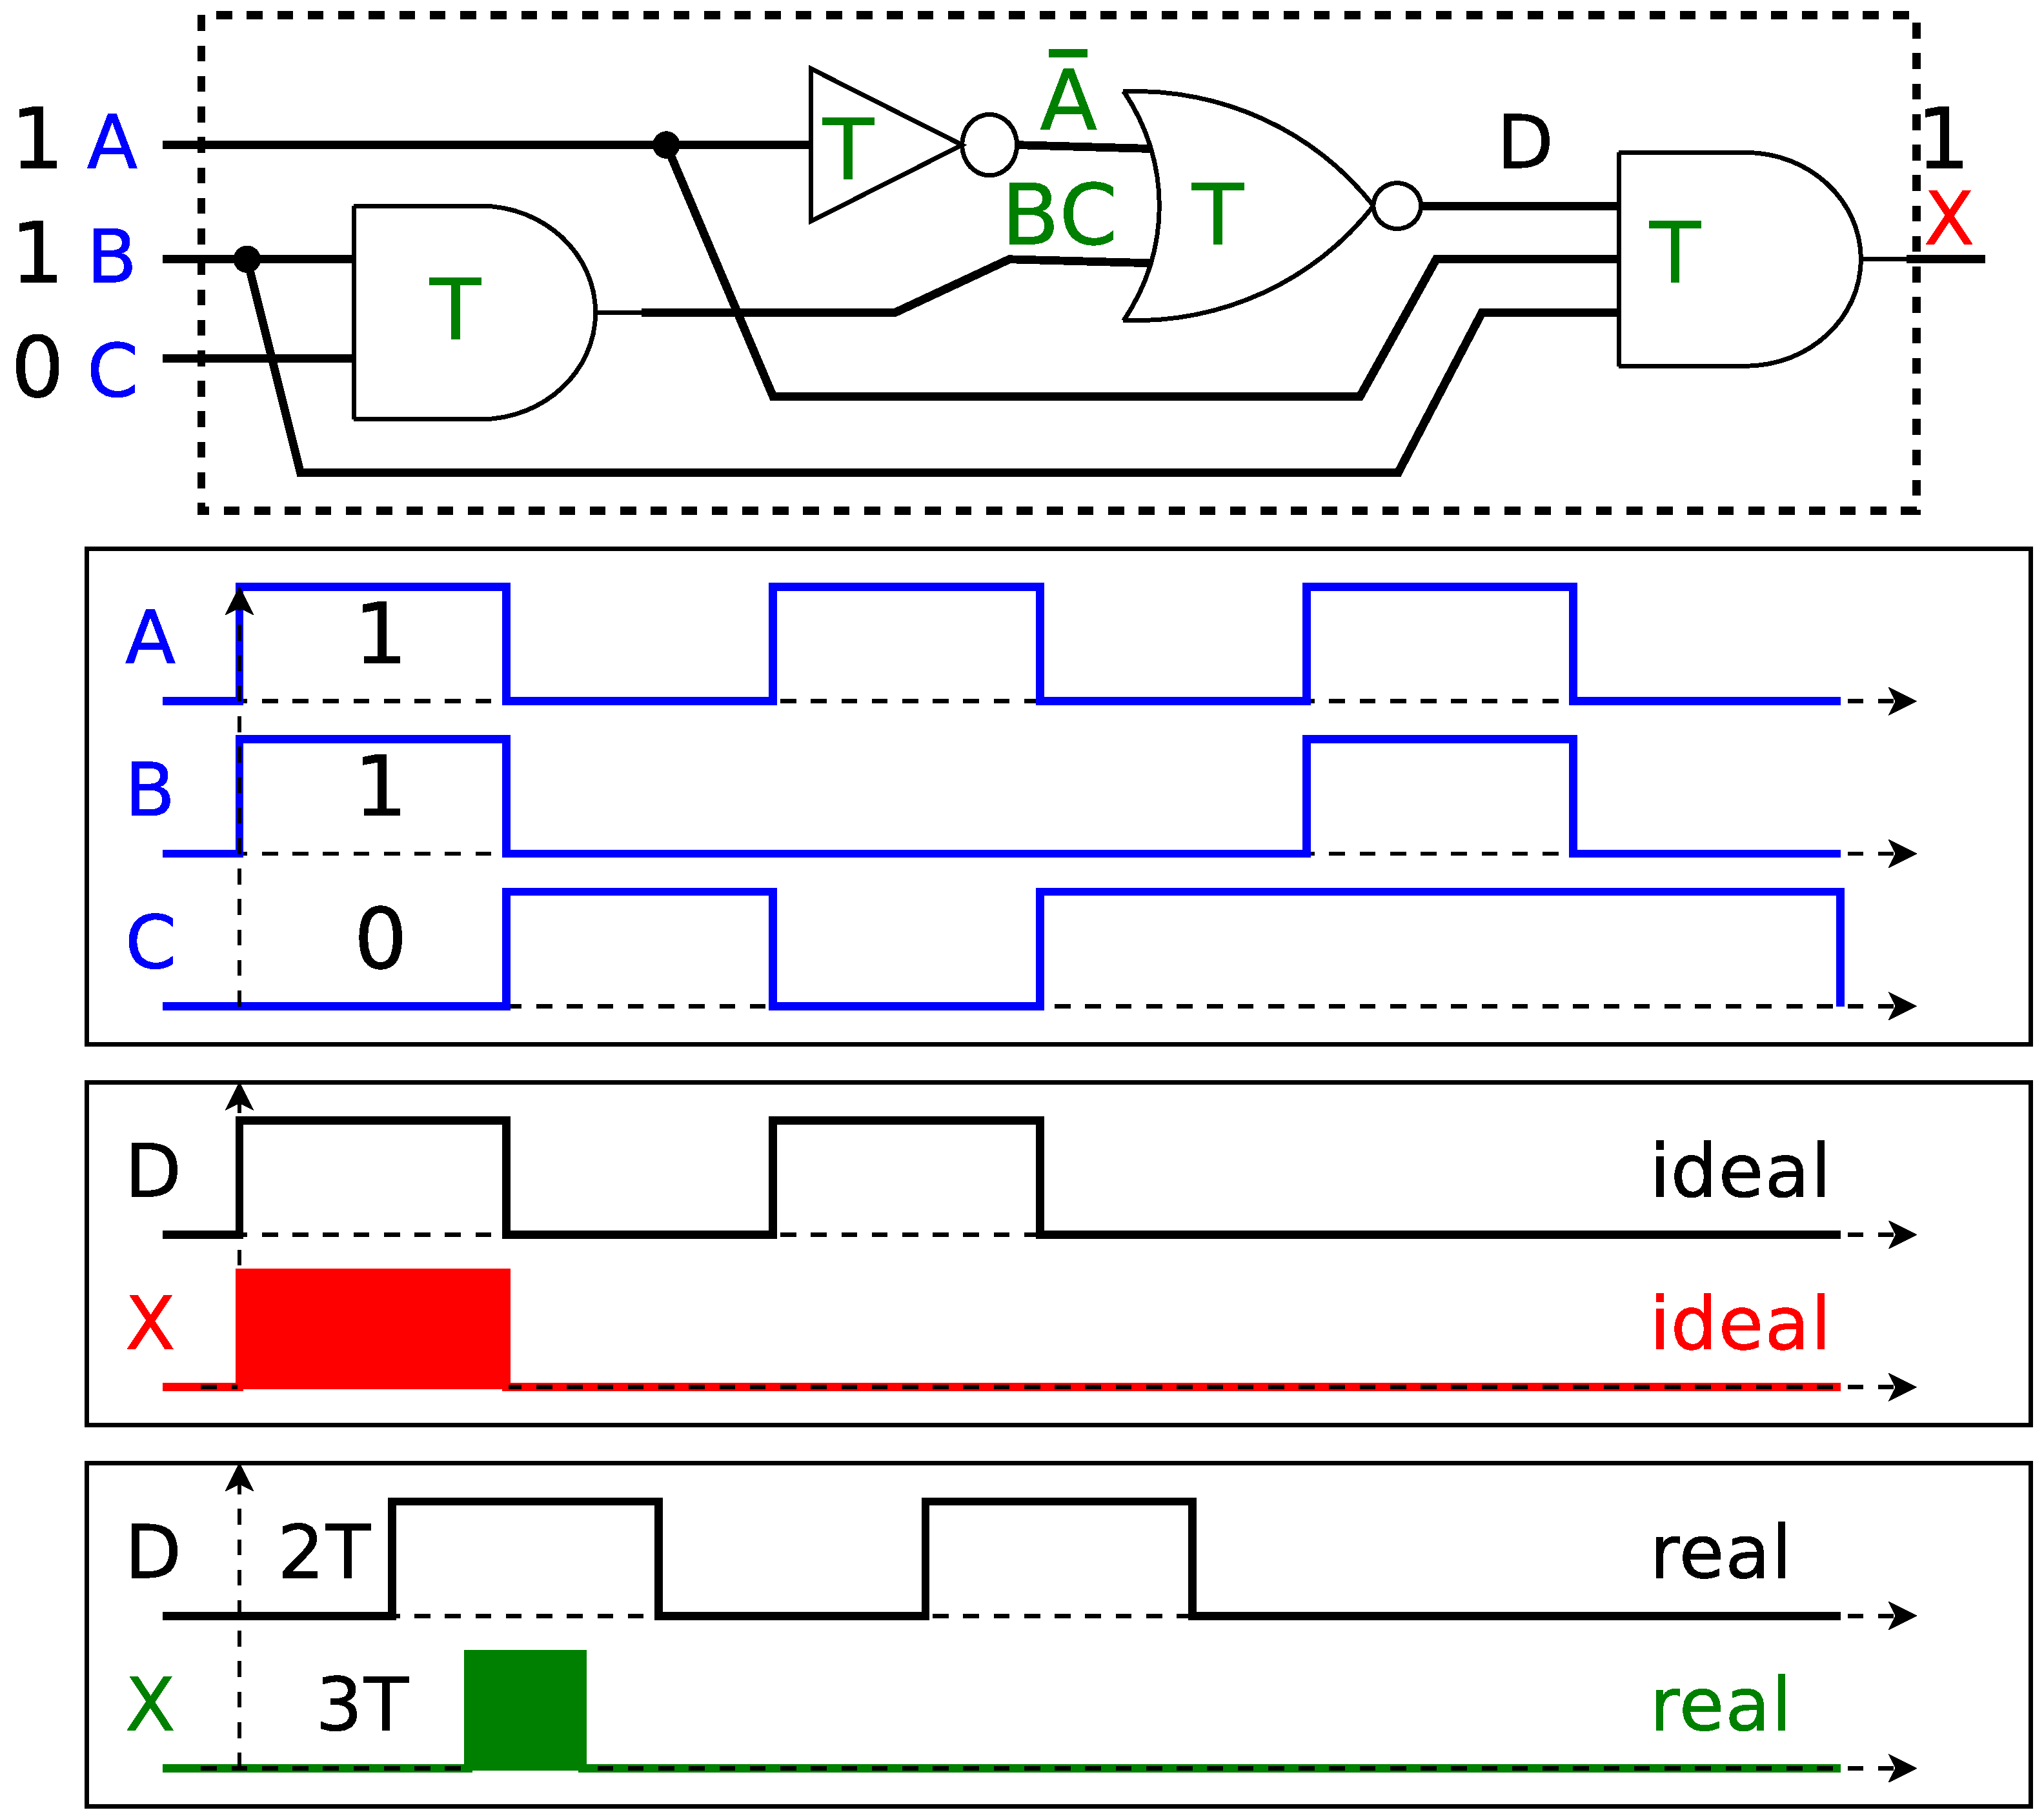
\includegraphics[width=0.7\textwidth]{images/combinacional.eps}
\end{center} 
\end{frame}

%%%%%%%%%%%%%%%%%%%%%%%%%%%%%%%%%%%%%%%%%%%%%%%%%%%%%%%%%%%%%%%%%%%%%%%%%%%%%%%%
\begin{frame}{Lógica sequencial}
\begin{center}
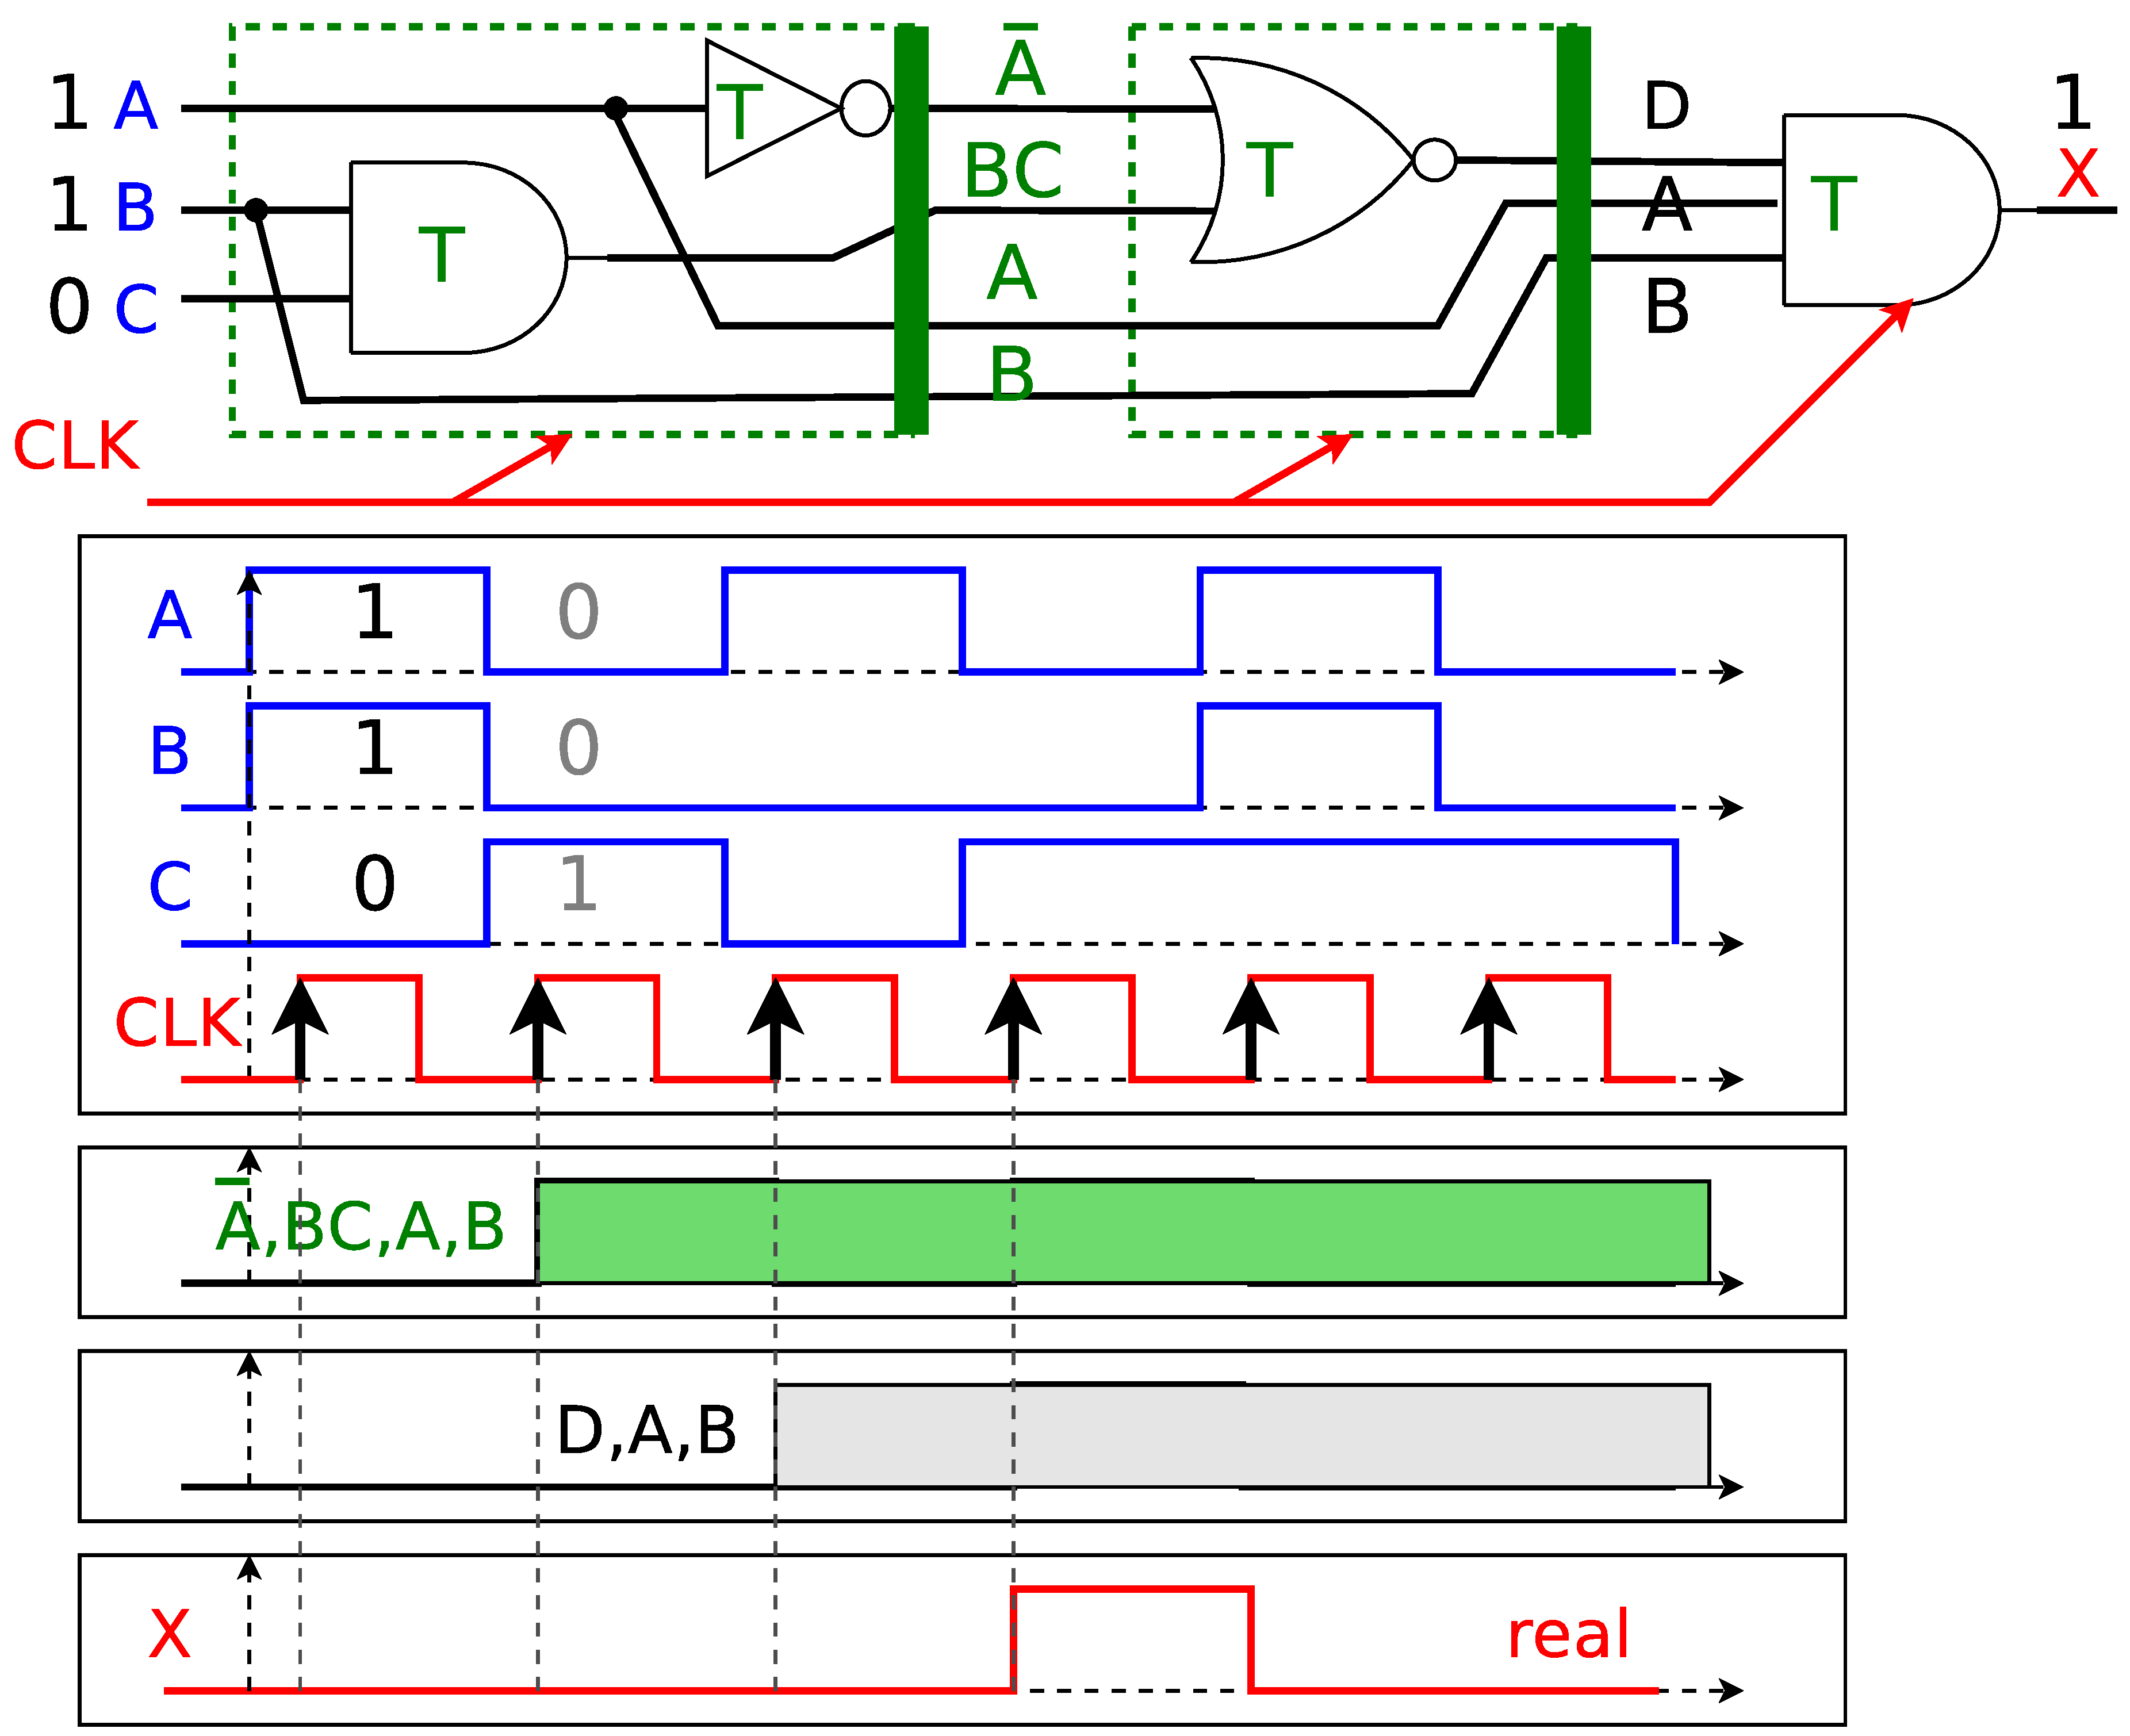
\includegraphics[width=0.8\textwidth]{images/combinacional2.eps}
\end{center} 
\end{frame}

%%%%%%%%%%%%%%%%%%%%%%%%%%%%%%%%%%%%%%%%%%%%%%%%%%%%%%%%%%%%%%%%%%%%%%%%%%%%%%%%
\begin{frame}{Lógica sequencial}
\begin{description}
 \item[Circuito combinacional] a saída depende exclusivamente da {\color{red}combinação de suas entradas}.
 \item[Circuito sequencial] a saída futura depende de sua {\color{red} saída atual} 
 e da da {\color{red}combinação de suas entradas}   
 (Armazena valores antigos).
\end{description}

O elemento de memória mais importante é o Flip-Flop.
\begin{center}
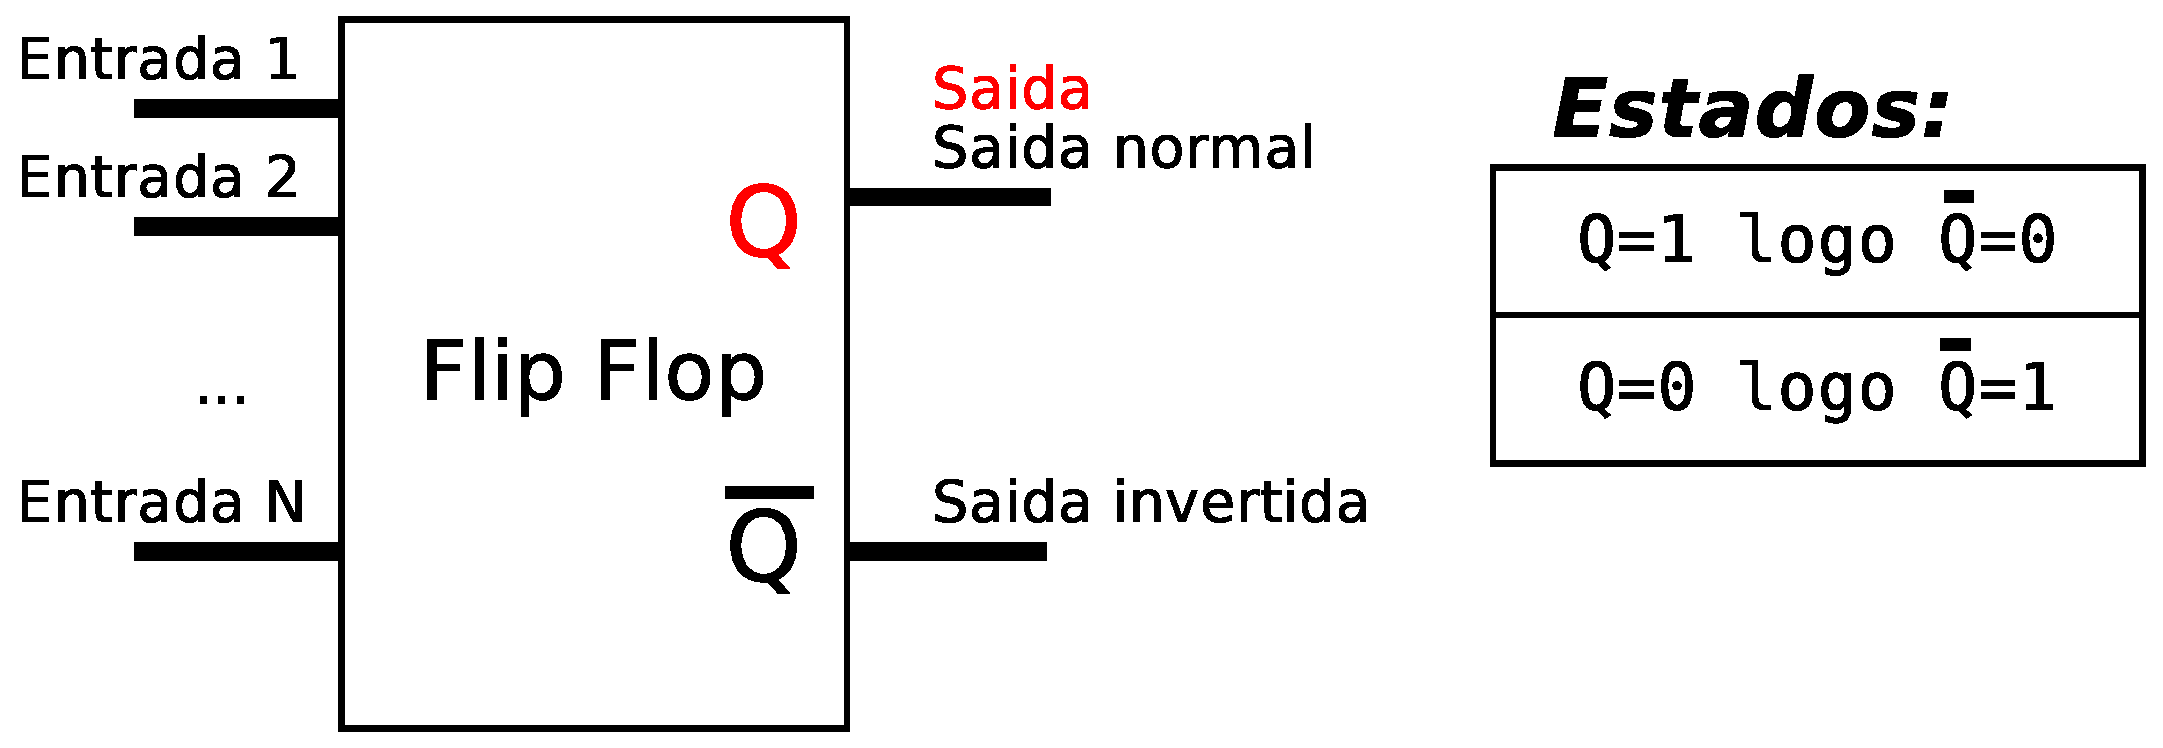
\includegraphics[width=0.7\textwidth]{images/flipflop.eps}
\end{center} 
\end{frame}


%%%%%%%%%%%%%%%%%%%%%%%%%%%%%%%%%%%%%%%%%%%%%%%%%%%%%%%%%%%%%%%%%%%%%%%%%%%%%%%%
%\begin{frame}{Flip-Flop básico - Latch SR (SET-RESET)}
%Usando portas NAND
%\begin{center}
%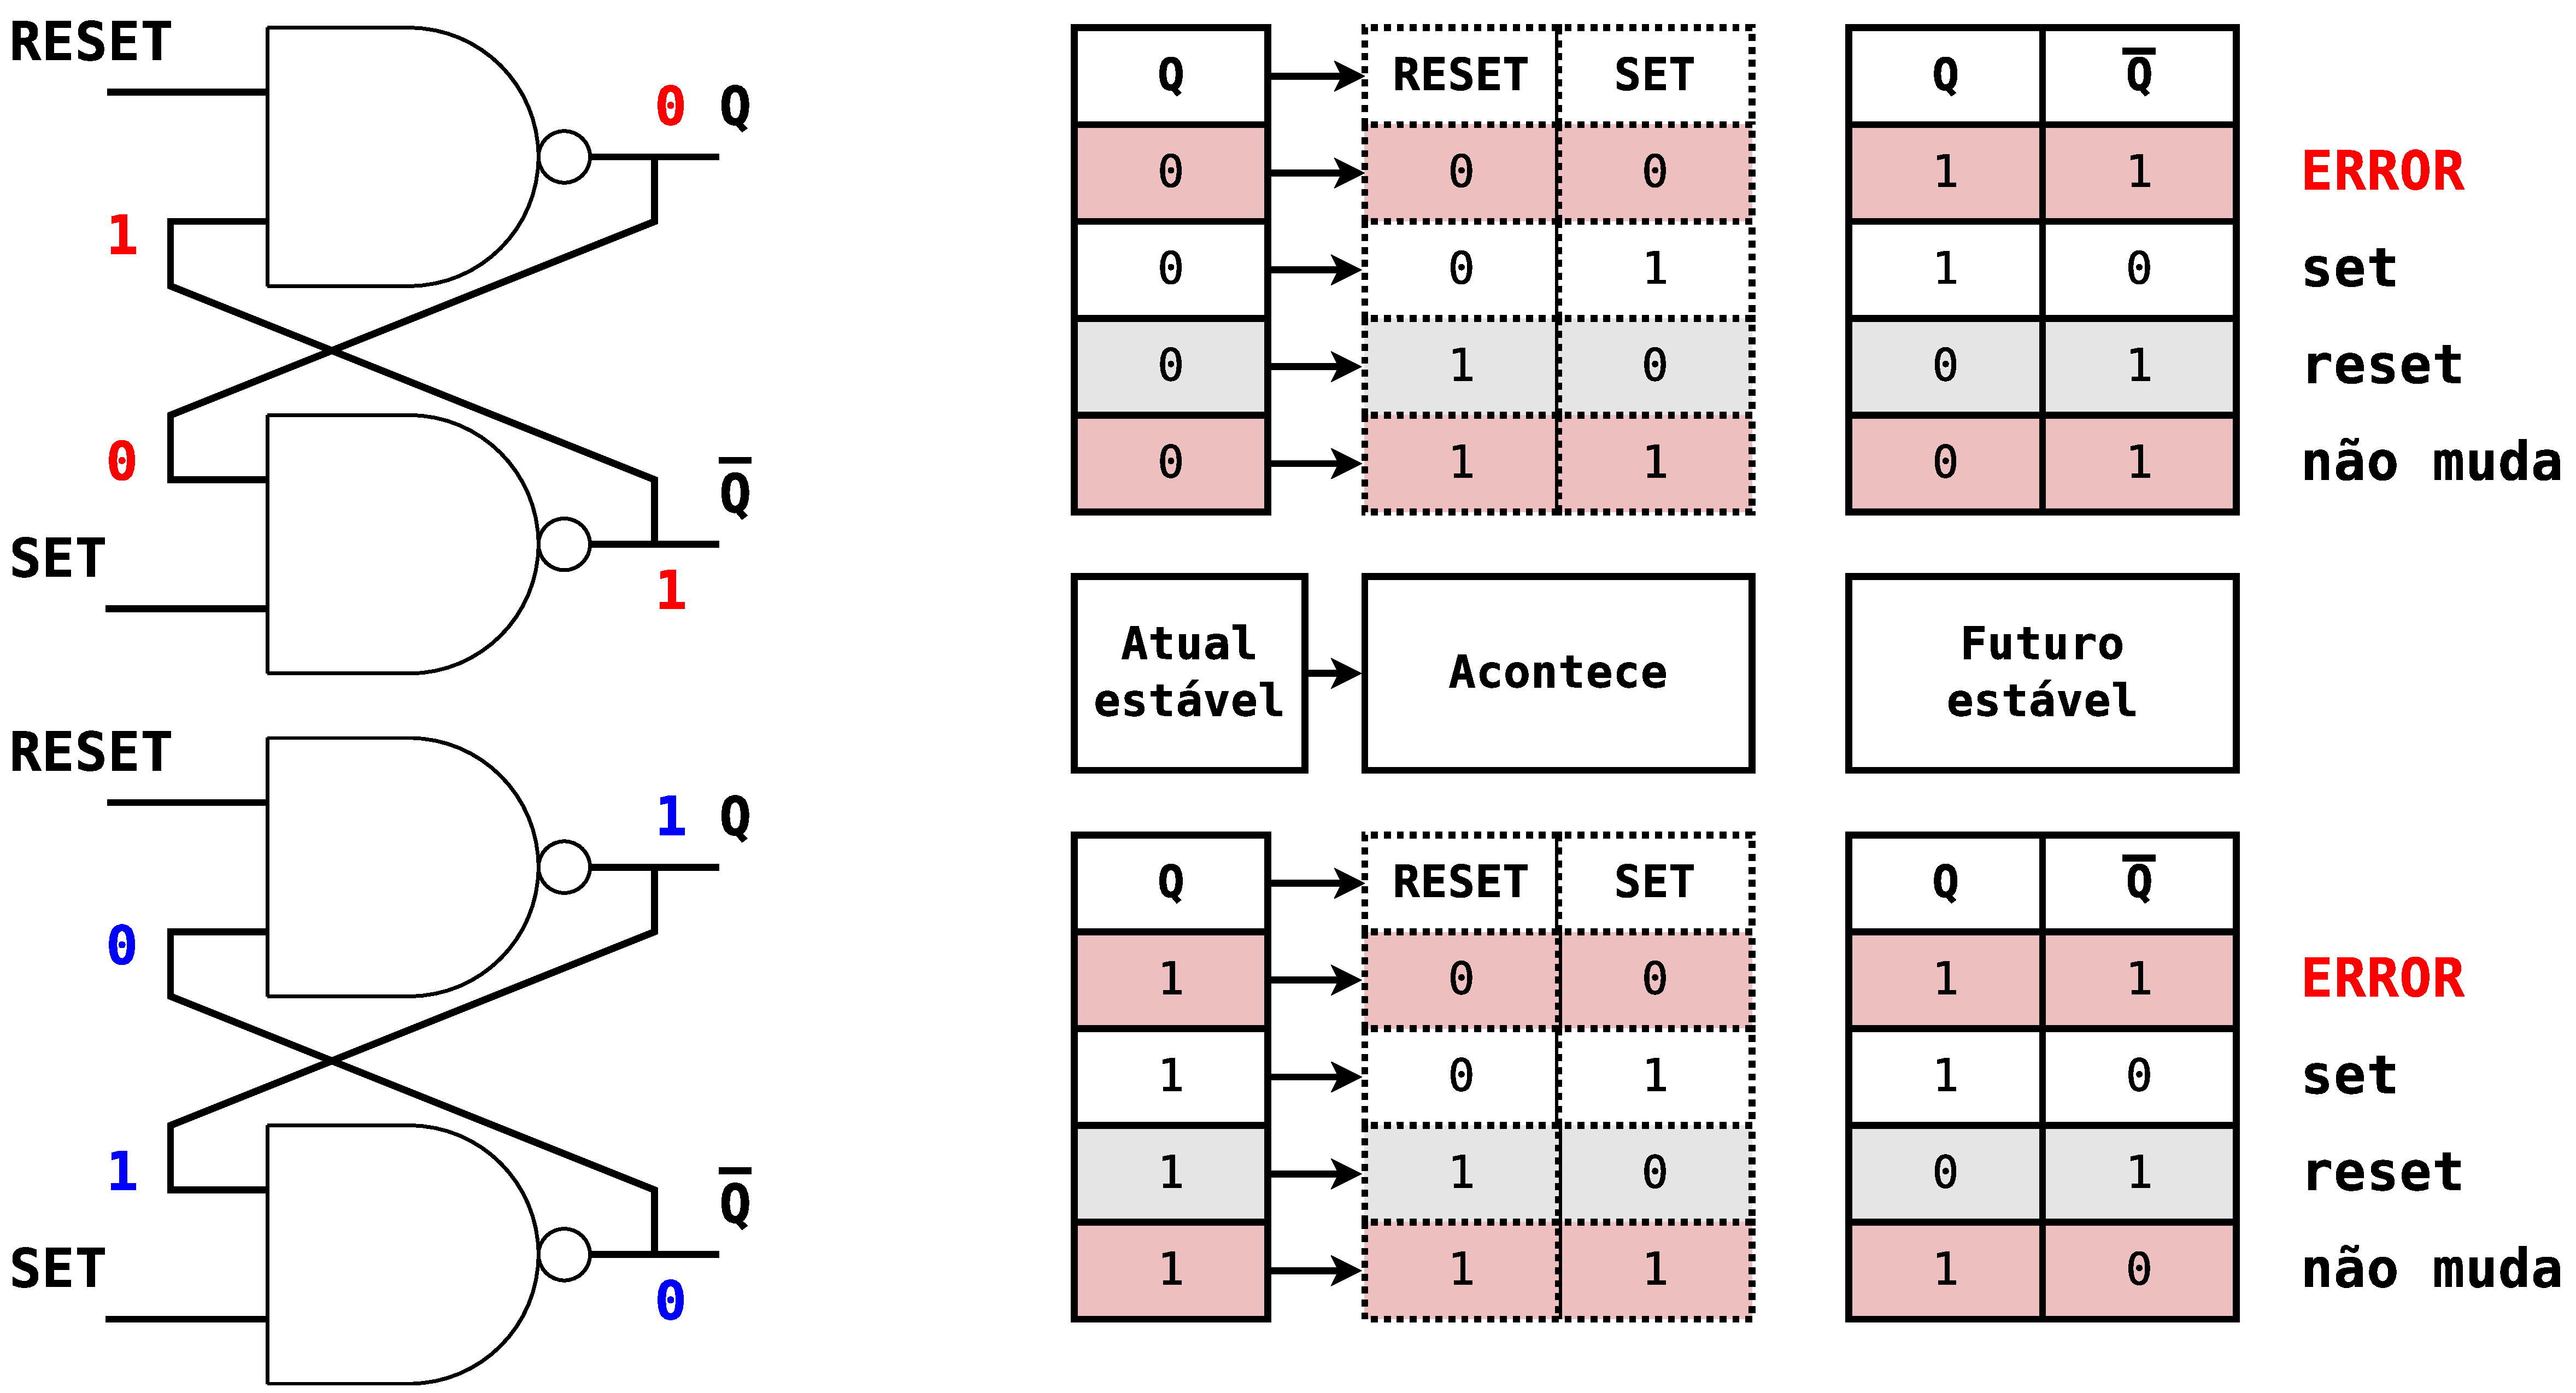
\includegraphics[width=0.9\textwidth]{images/nandlatch.eps}
%\end{center} 
%\end{frame}


%%%%%%%%%%%%%%%%%%%%%%%%%%%%%%%%%%%%%%%%%%%%%%%%%%%%%%%%%%%%%%%%%%%%%%%%%%%%%%%%
\begin{frame}{Flip-Flop básico - SR NAND LATCH (SET-RESET)}
Usando portas NAND
\begin{center}
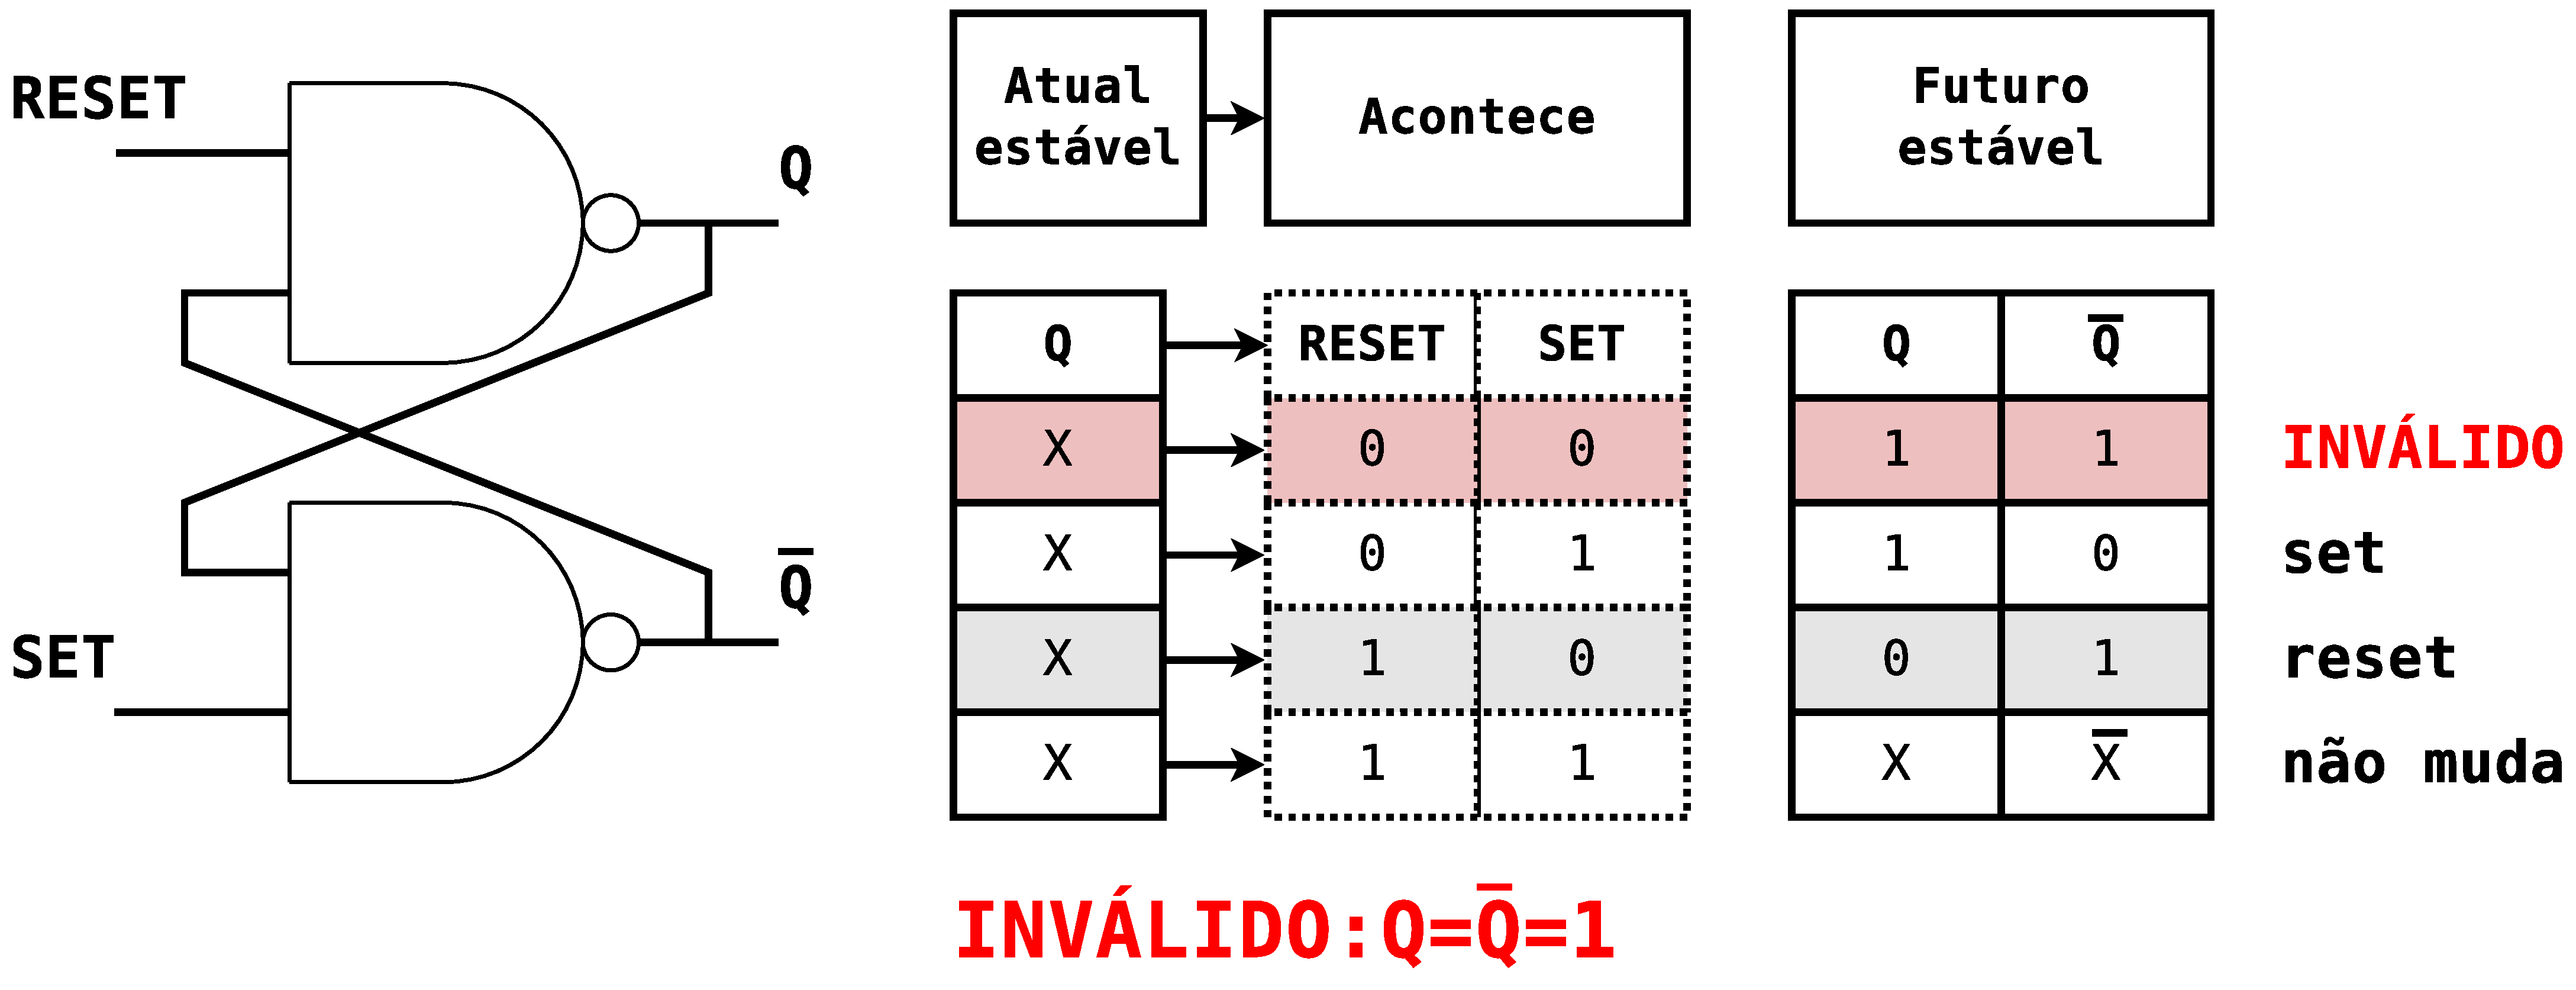
\includegraphics[width=0.9\textwidth]{images/nandlatch2.eps}
\end{center} 
\end{frame}

%%%%%%%%%%%%%%%%%%%%%%%%%%%%%%%%%%%%%%%%%%%%%%%%%%%%%%%%%%%%%%%%%%%%%%%%%%%%%%%%
\begin{frame}{Flip-Flop básico - SR NOR LATCH (SET-RESET)}
Usando portas NOR
\begin{center}
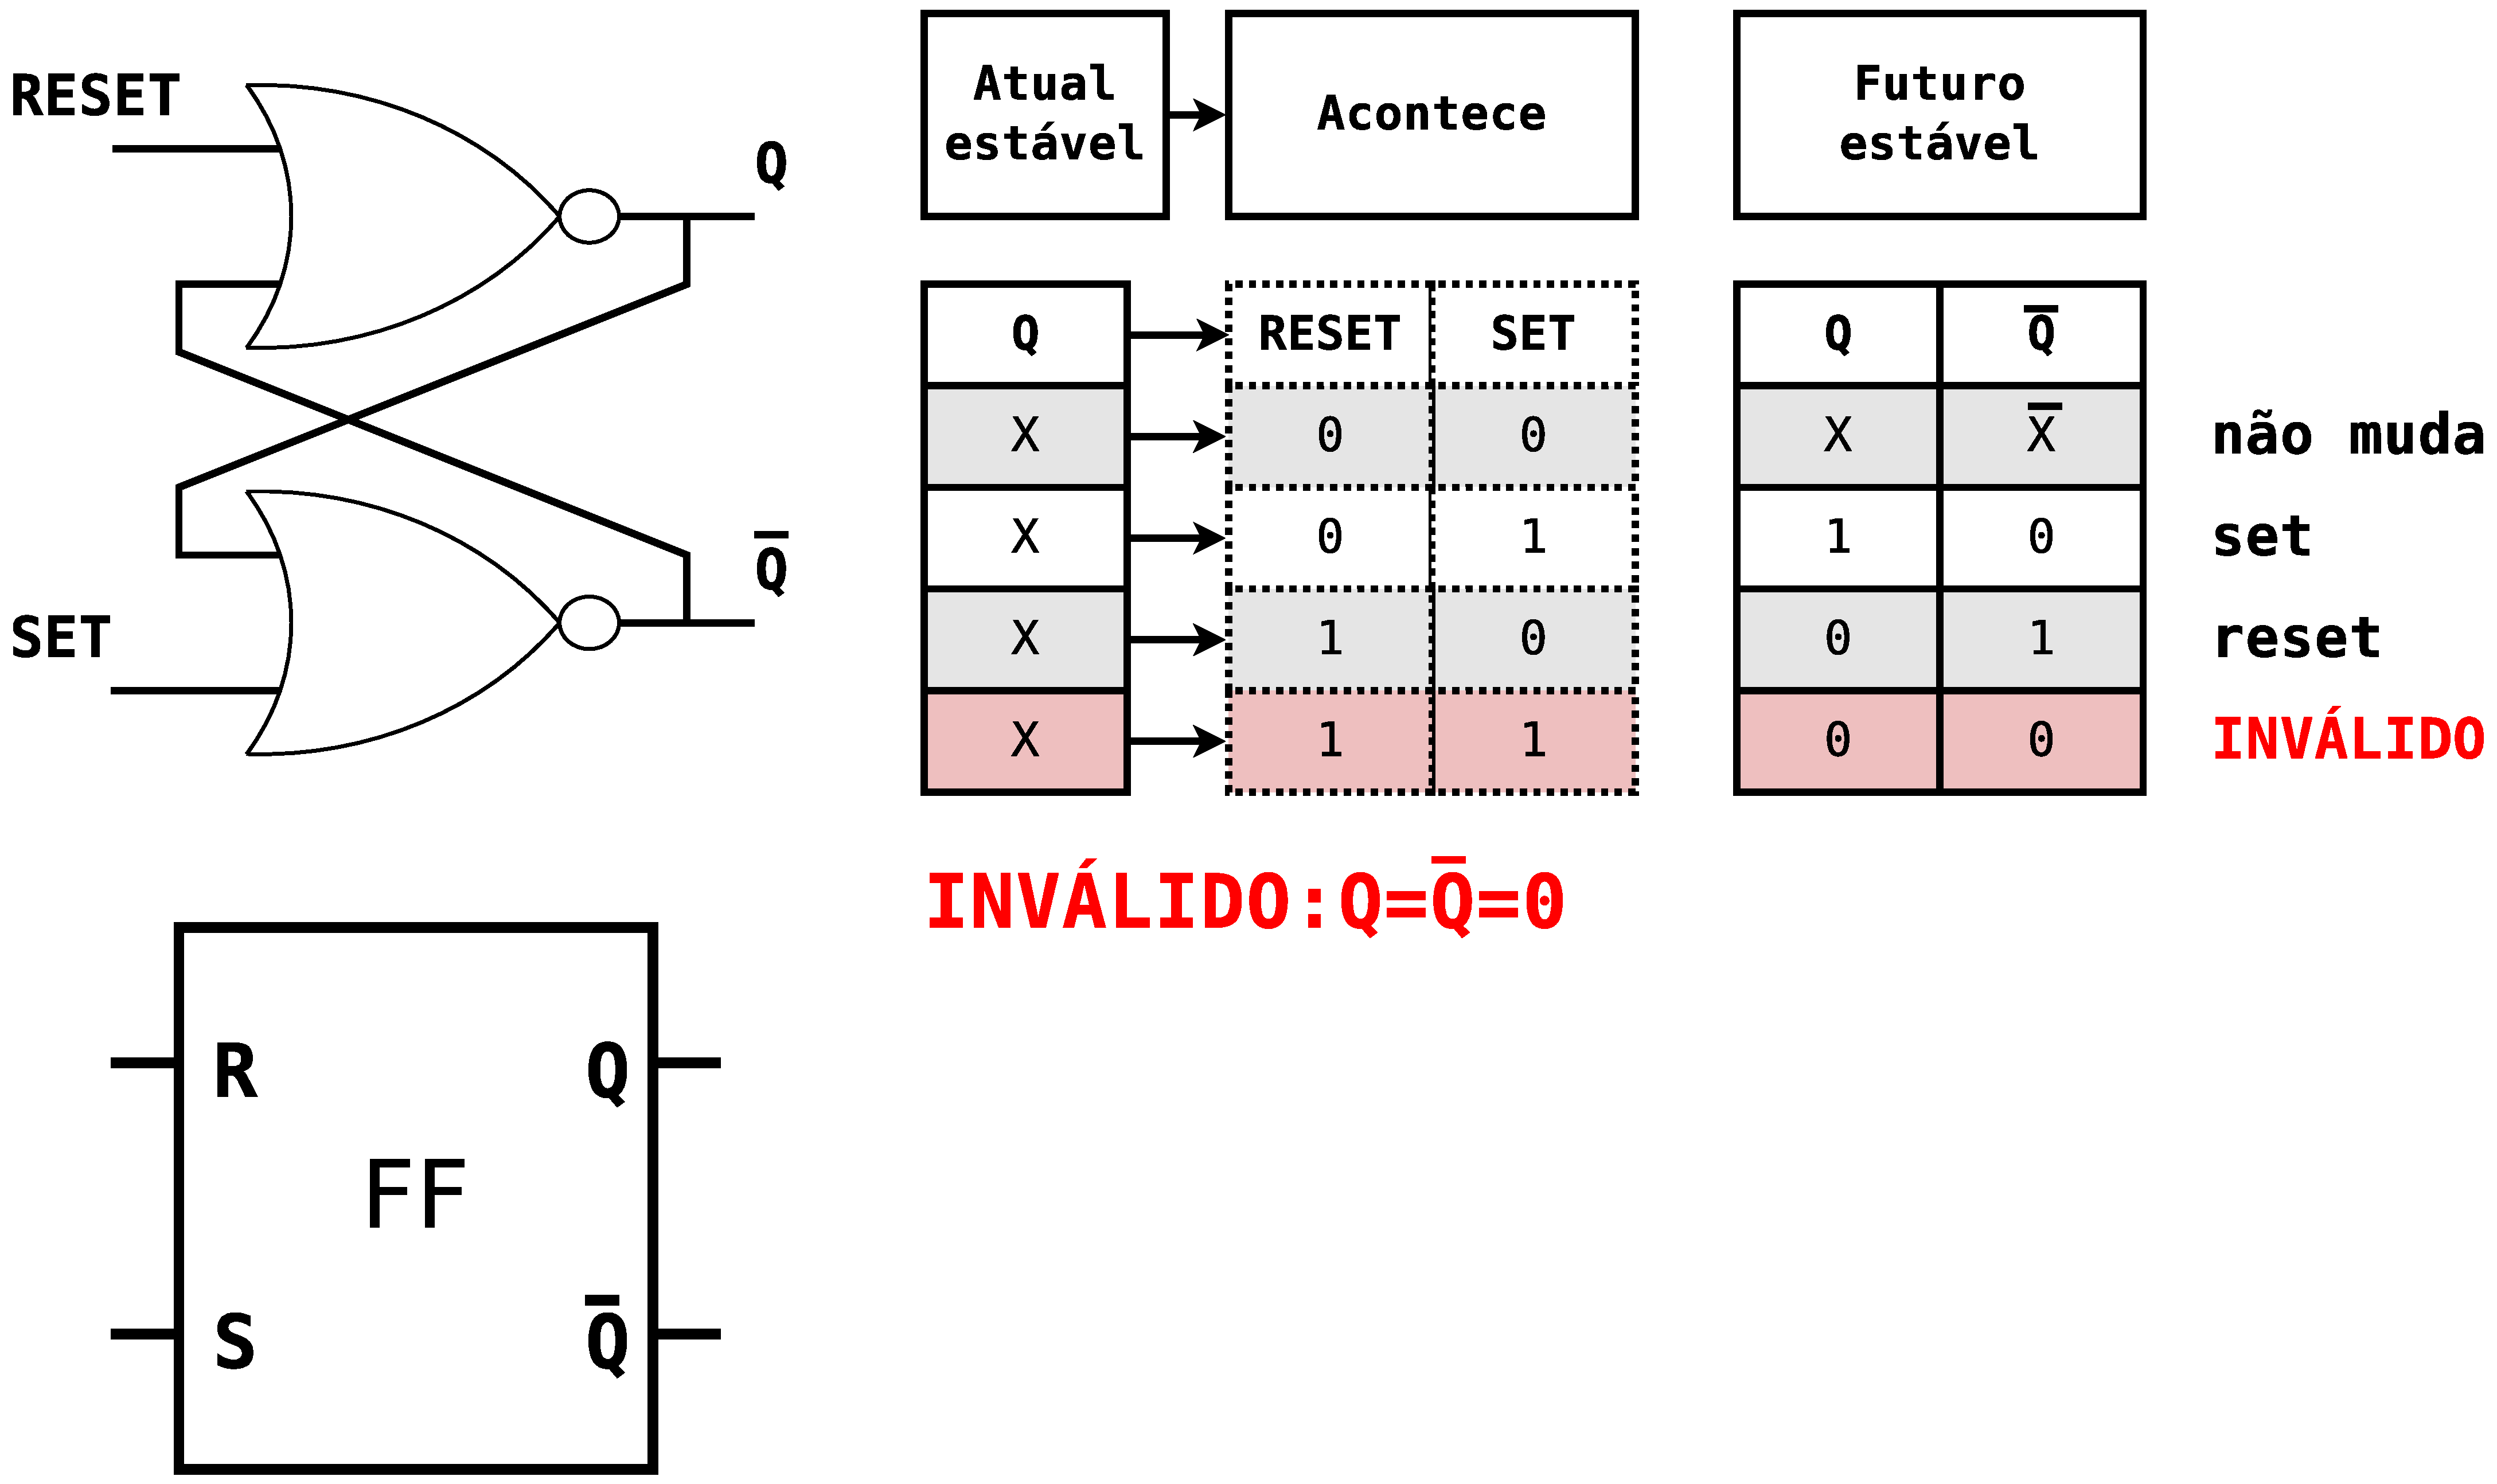
\includegraphics[width=0.9\textwidth]{images/norlatch2.eps}
\end{center} 
\end{frame}

%%%%%%%%%%%%%%%%%%%%%%%%%%%%%%%%%%%%%%%%%%%%%%%%%%%%%%%%%%%%%%%%%%%%%%%%%%%%%%%%
\begin{frame}{Flip-Flop básico - SR NOR LATCH (SET-RESET)}
Usando portas NOR
\begin{center}
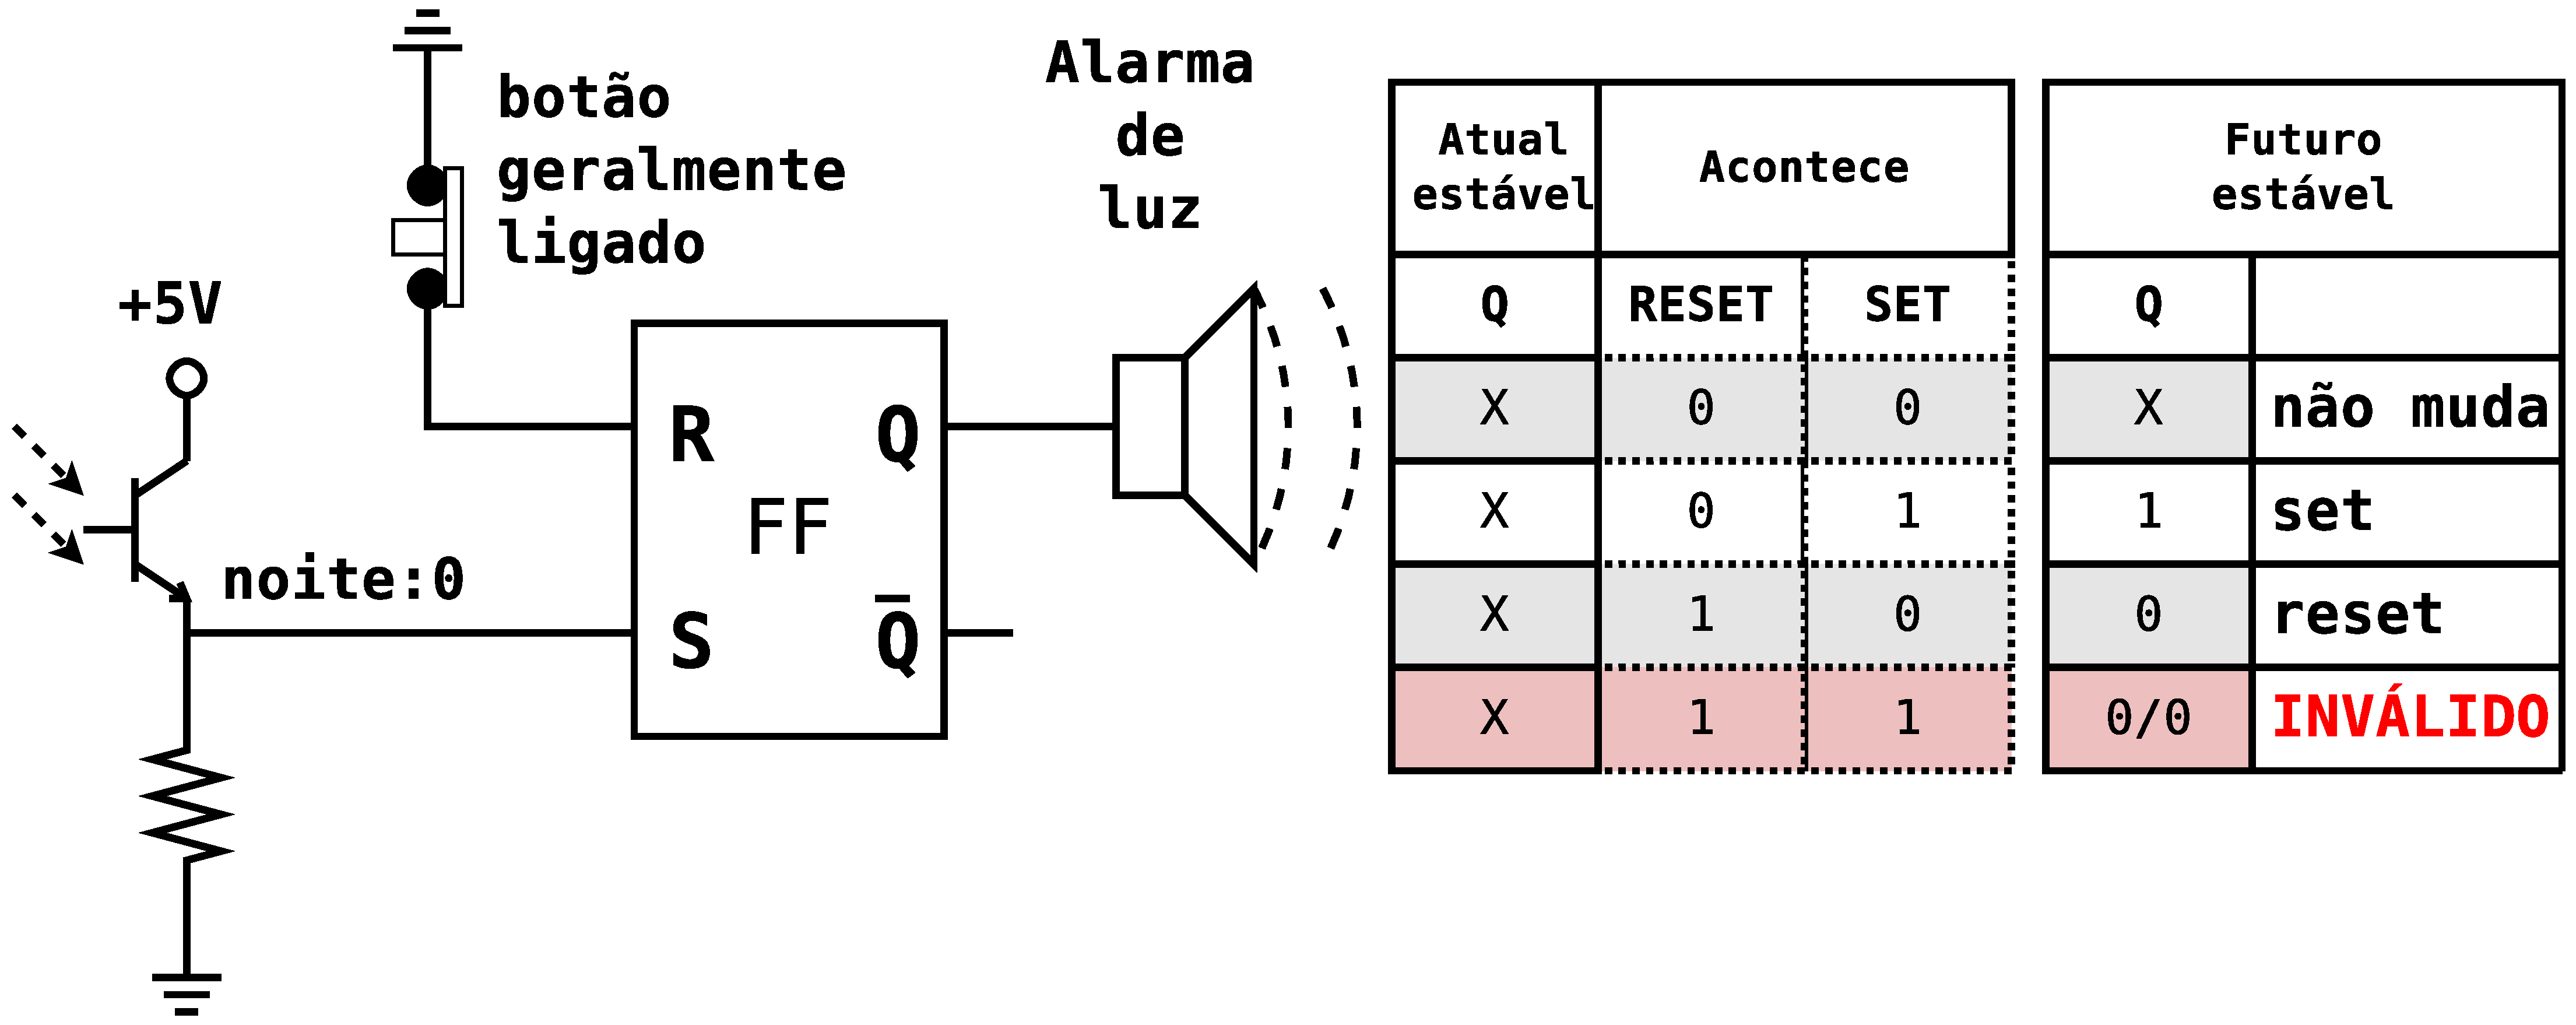
\includegraphics[width=0.99\textwidth]{images/norlatch3.eps}
\end{center} 
\end{frame}

%%%%%%%%%%%%%%%%%%%%%%%%%%%%%%%%%%%%%%%%%%%%%%%%%%%%%%%%%%%%%%%%%%%%%%%%%%%%%%%%
\begin{frame}{Flip-Flop com CLOCK}
\begin{center}
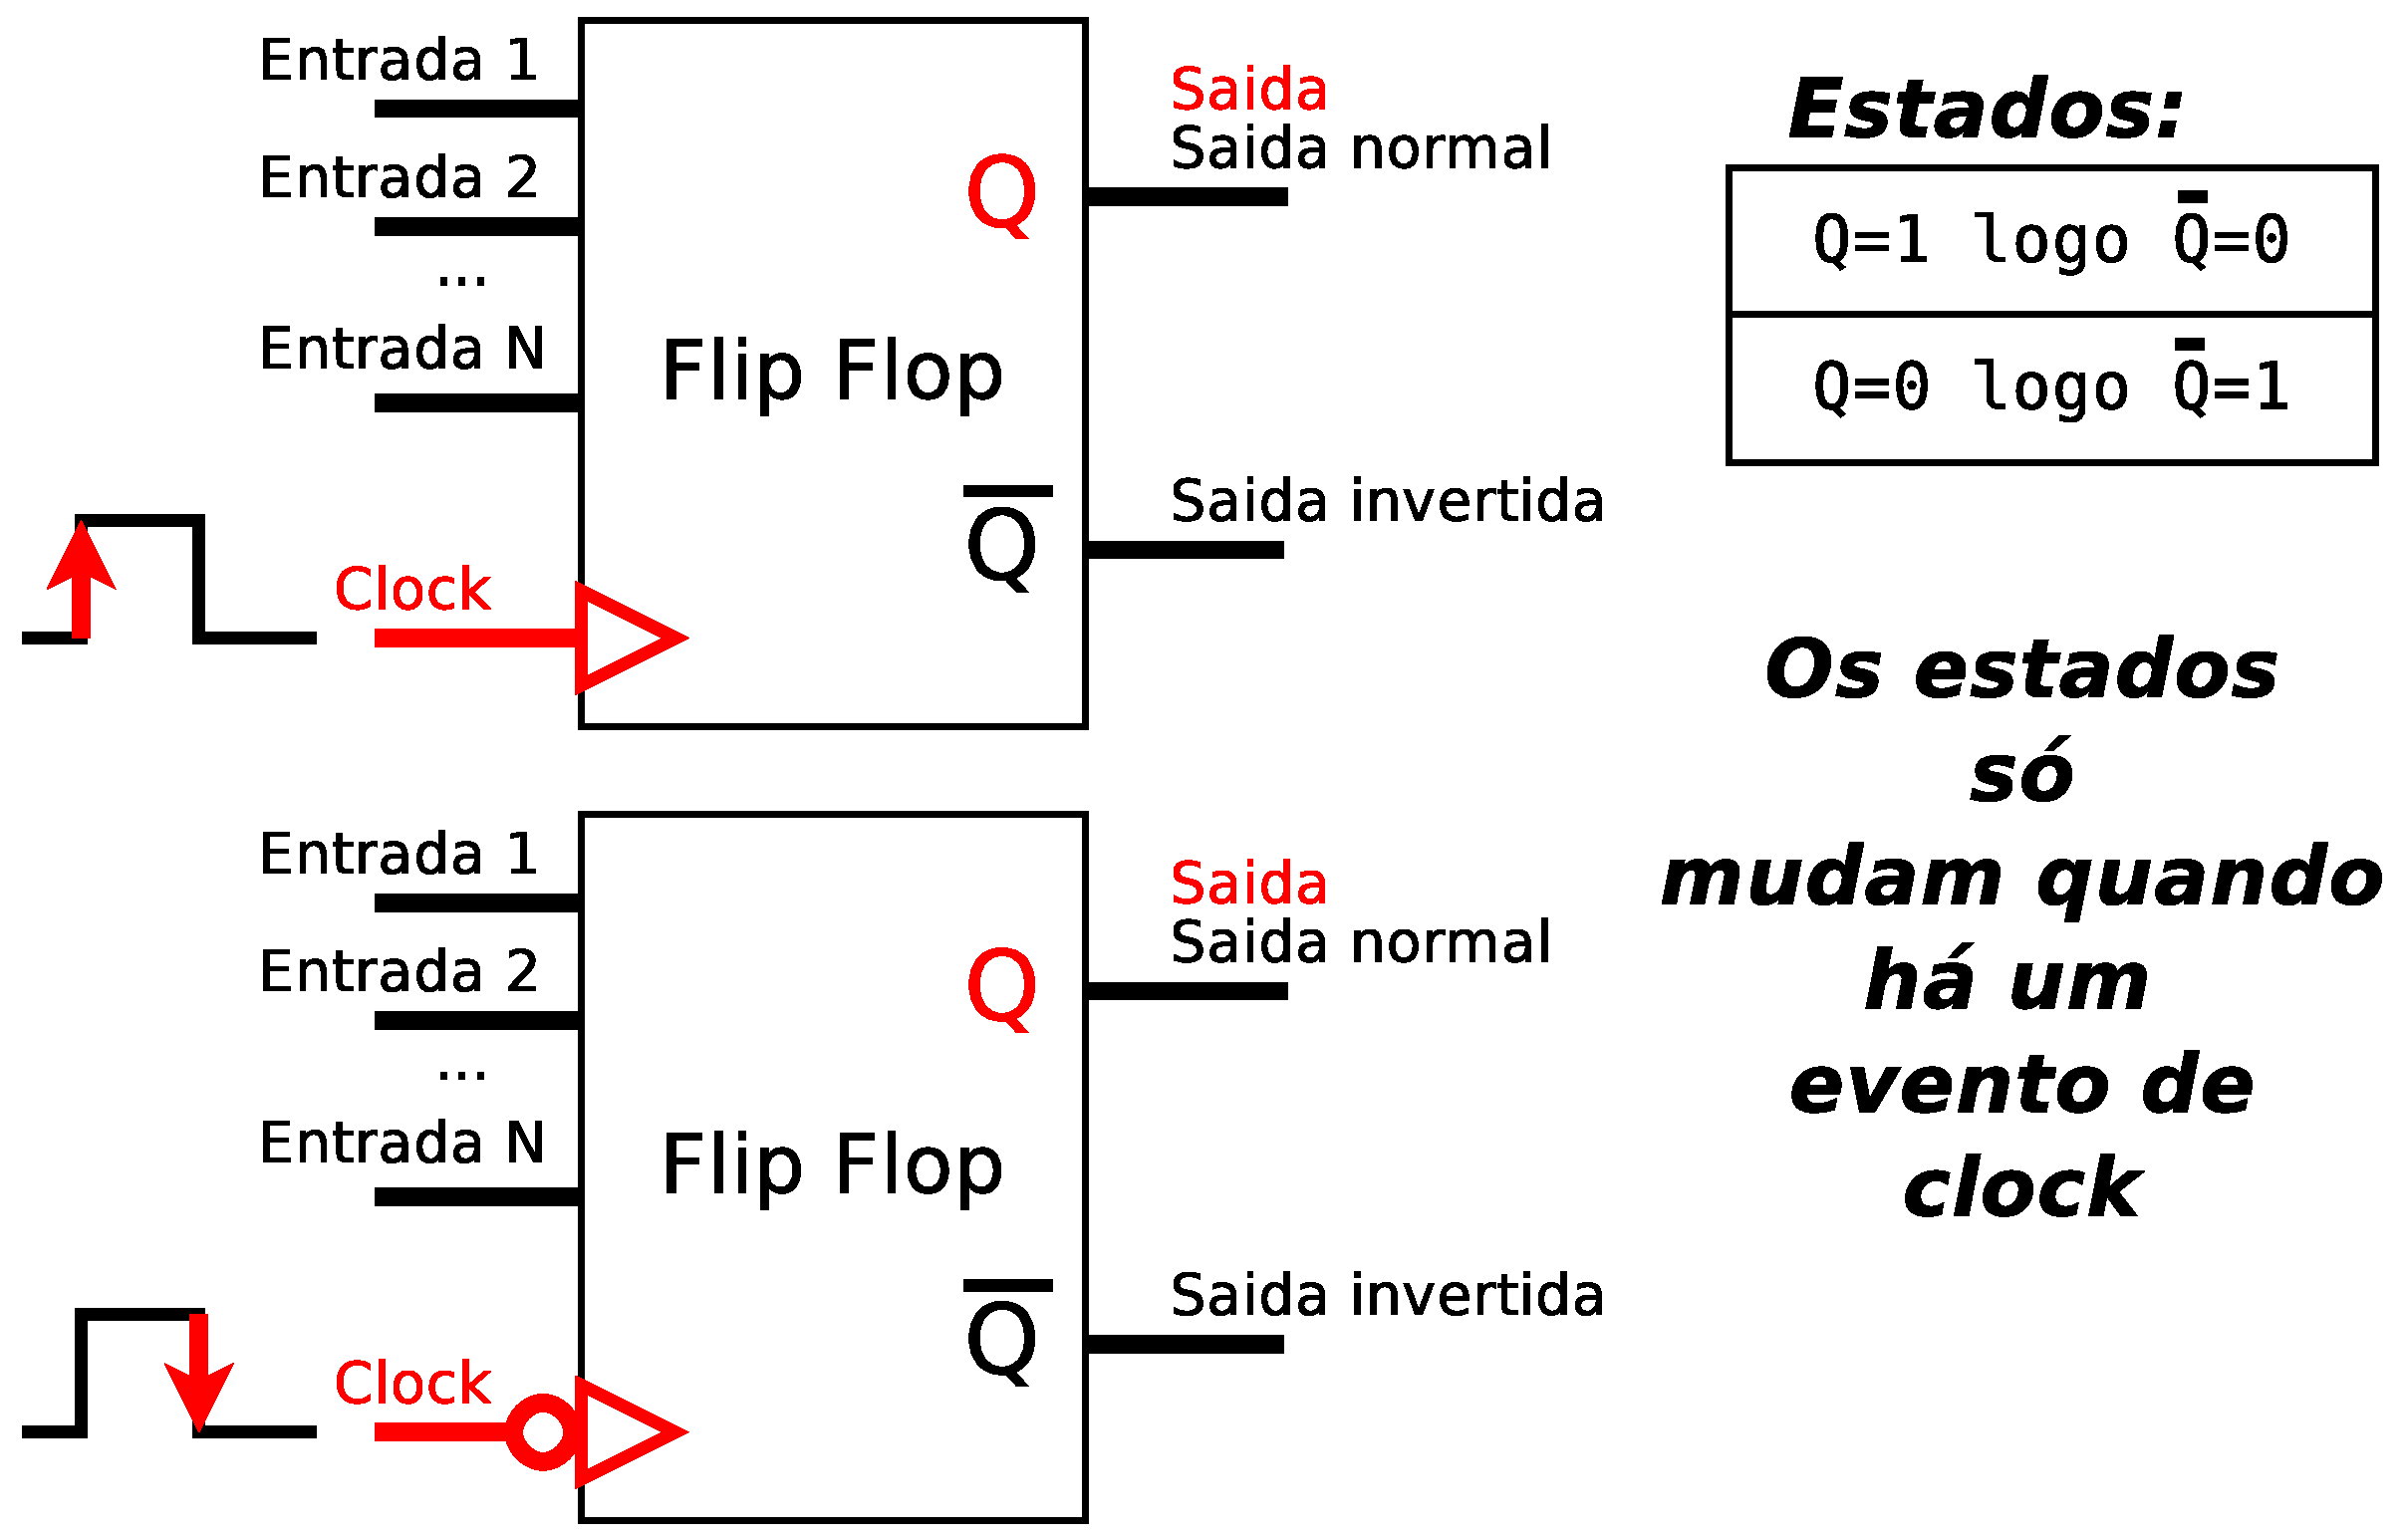
\includegraphics[width=0.9\textwidth]{images/flipflopclock.eps}
\end{center} 
\end{frame}

%%%%%%%%%%%%%%%%%%%%%%%%%%%%%%%%%%%%%%%%%%%%%%%%%%%%%%%%%%%%%%%%%%%%%%%%%%%%%%%%
\begin{frame}{Flip-Flop SR NAND com CLOCK}
Usando portas NAND
\begin{center}
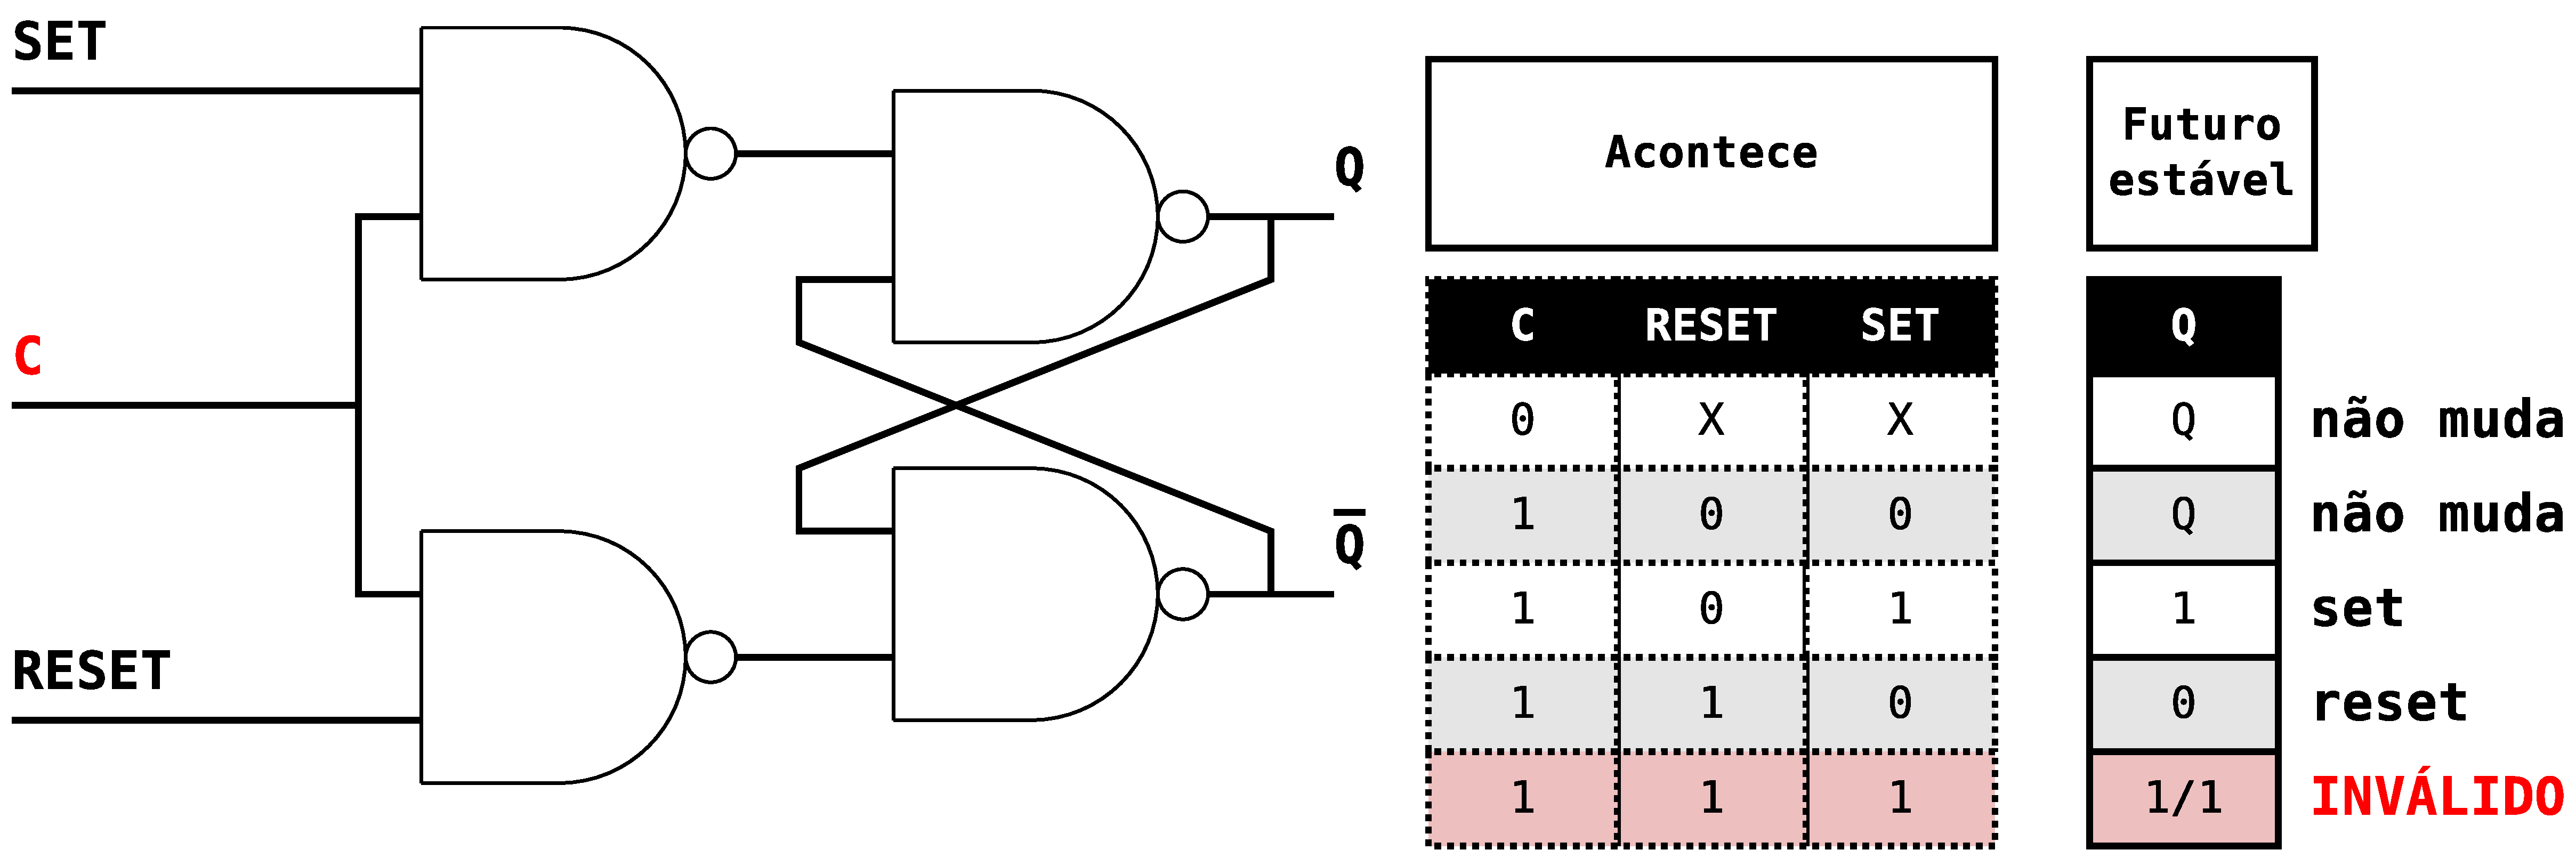
\includegraphics[width=0.99\textwidth]{images/nandclk.eps}
\end{center} 
\end{frame}

%%%%%%%%%%%%%%%%%%%%%%%%%%%%%%%%%%%%%%%%%%%%%%%%%%%%%%%%%%%%%%%%%%%%%%%%%%%%%%%%
\begin{frame}{Detetor de transição }
\begin{center}
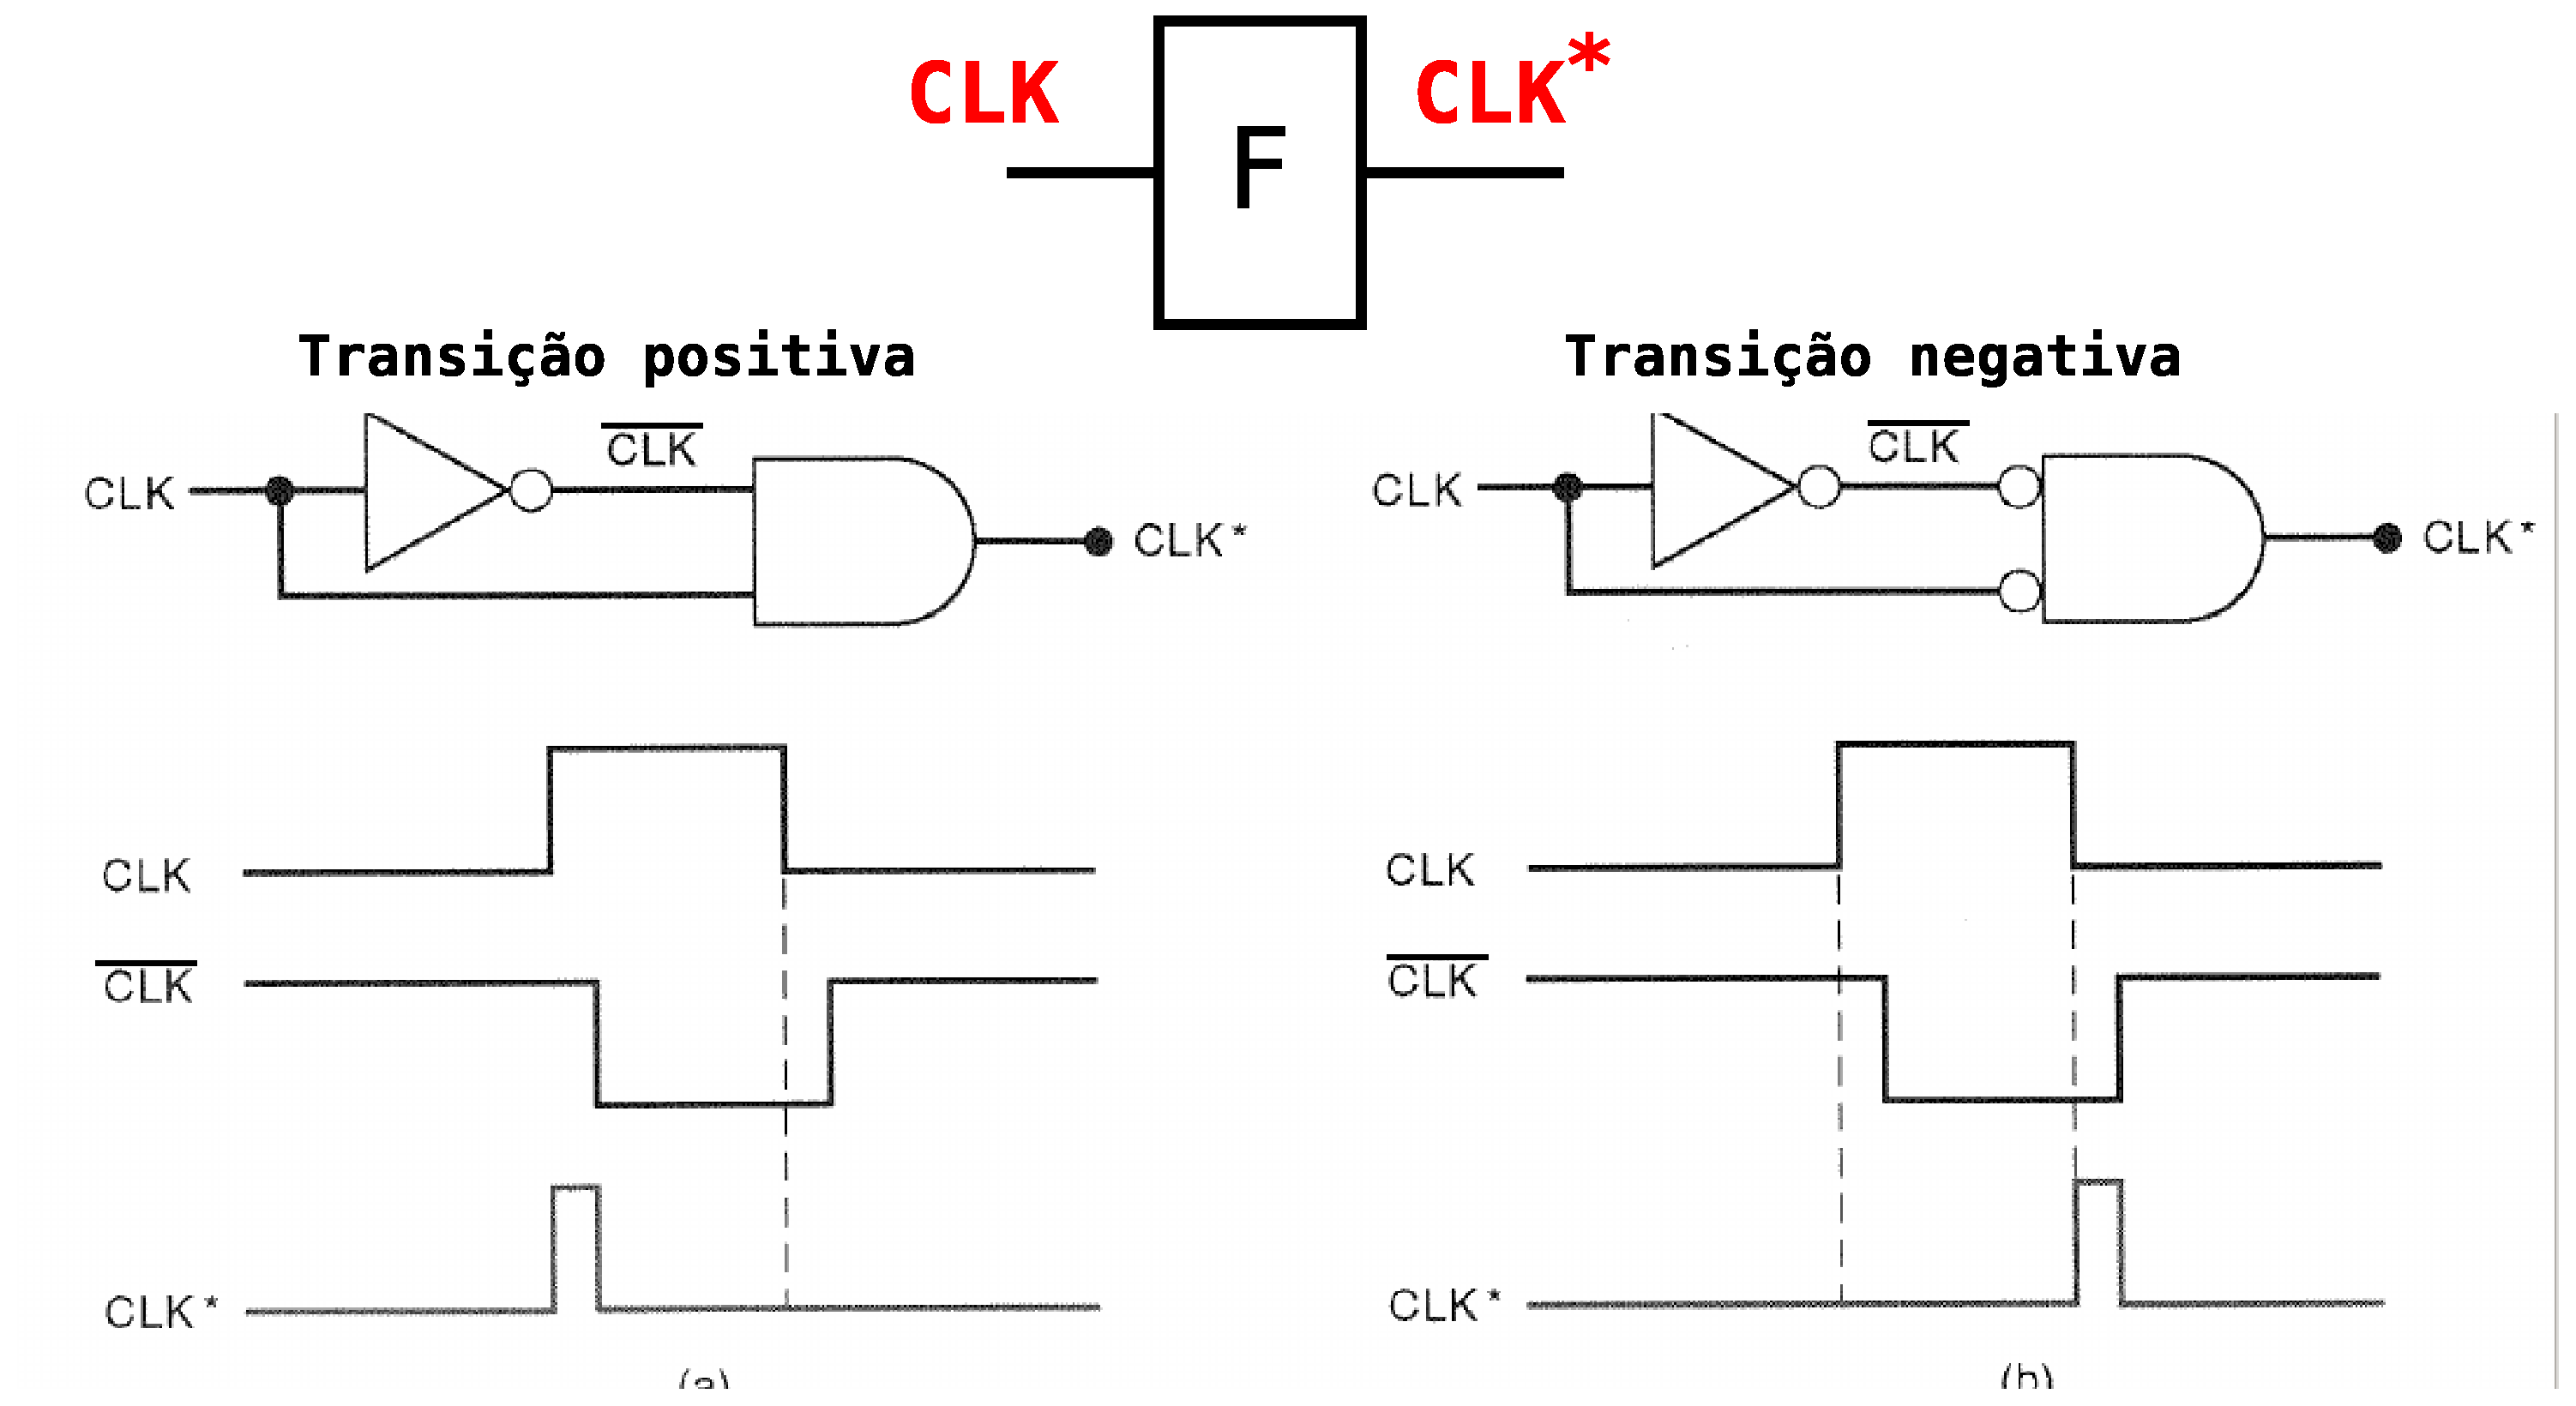
\includegraphics[width=0.99\textwidth]{images/Ftrans1.eps}
\end{center} 
\end{frame}


%%%%%%%%%%%%%%%%%%%%%%%%%%%%%%%%%%%%%%%%%%%%%%%%%%%%%%%%%%%%%%%%%%%%%%%%%%%%%%%%
\begin{frame}{Flip-Flop SR NAND com CLOCK}
Usando portas NAND
\begin{center}
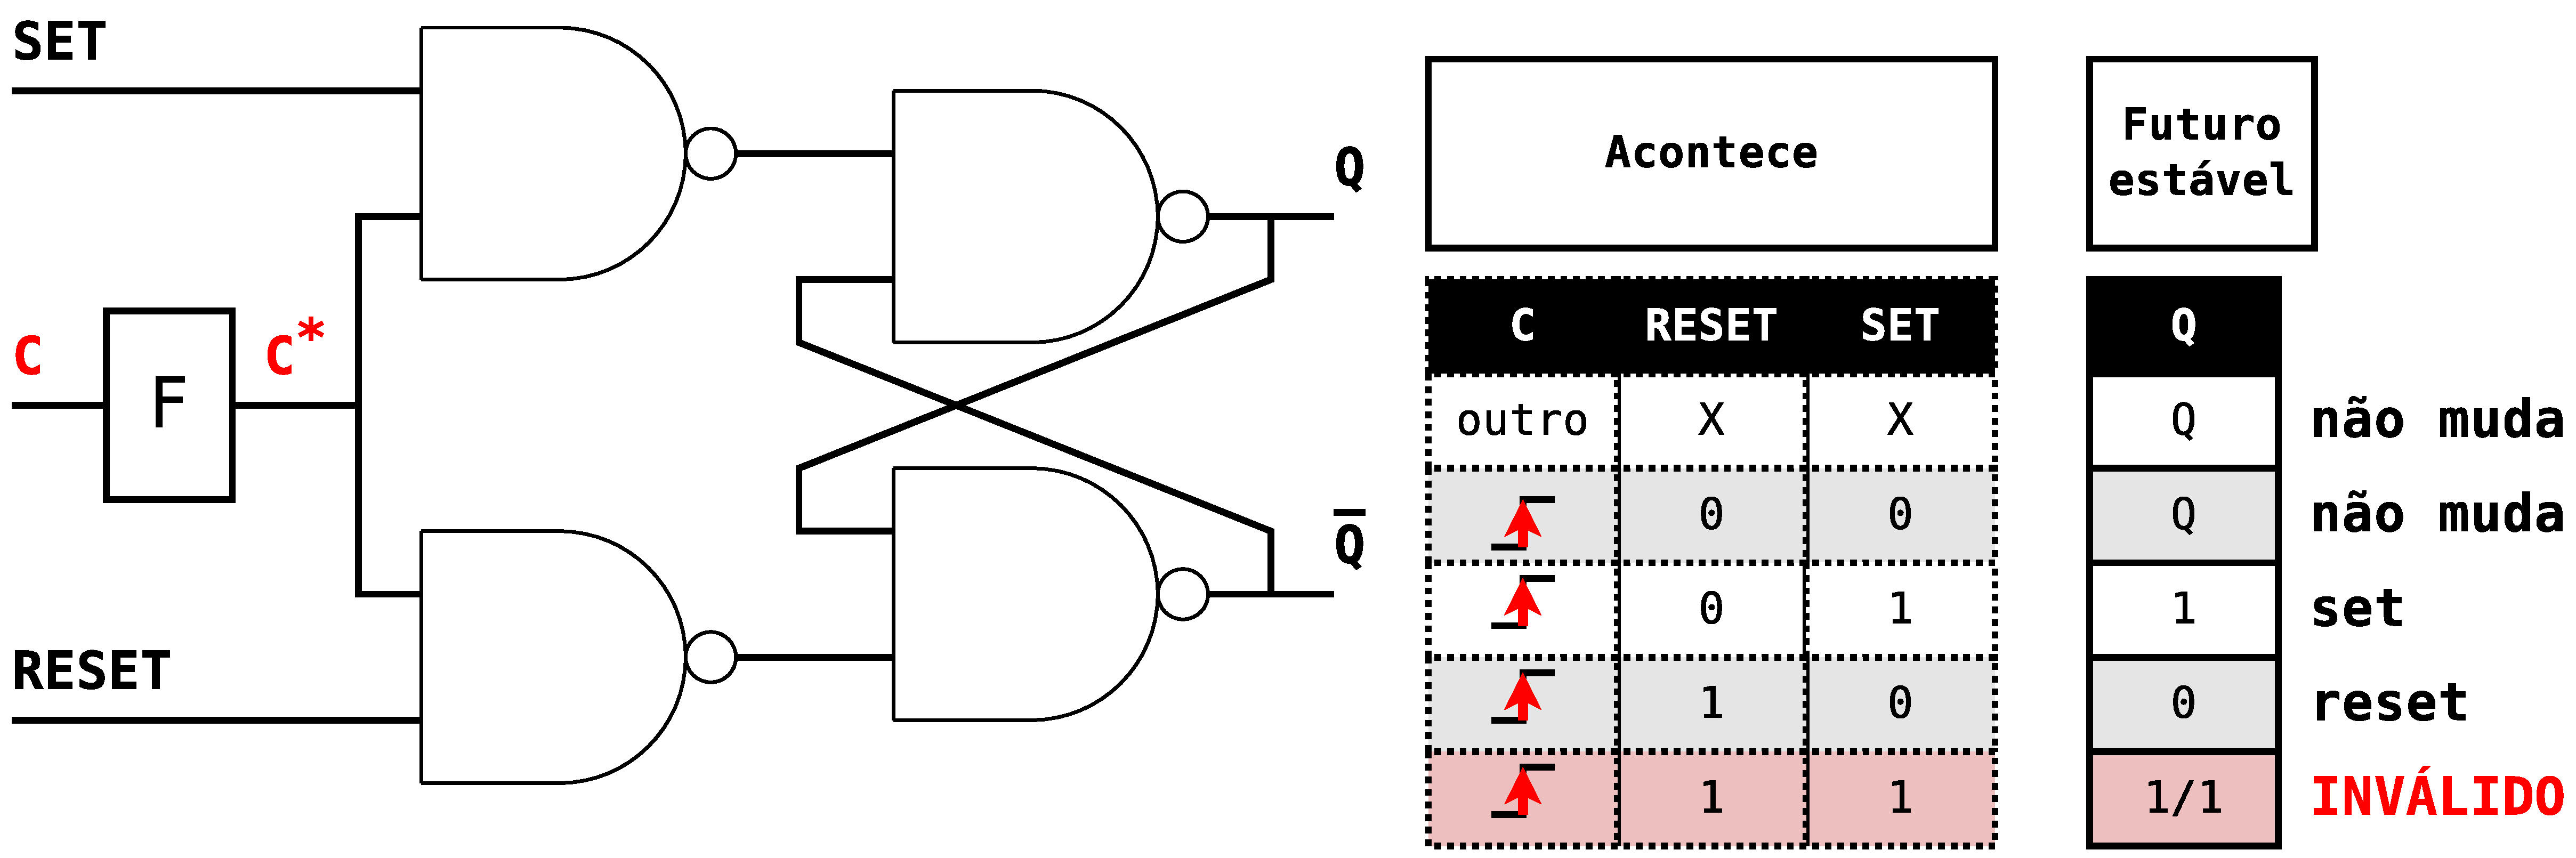
\includegraphics[width=0.99\textwidth]{images/nandclk2.eps}
\end{center} 
\end{frame}

%%%%%%%%%%%%%%%%%%%%%%%%%%%%%%%%%%%%%%%%%%%%%%%%%%%%%%%%%%%%%%%%%%%%%%%%%%%%%%%%
\begin{frame}{Flip-Flop JK}
Usando portas NAND
\begin{center}
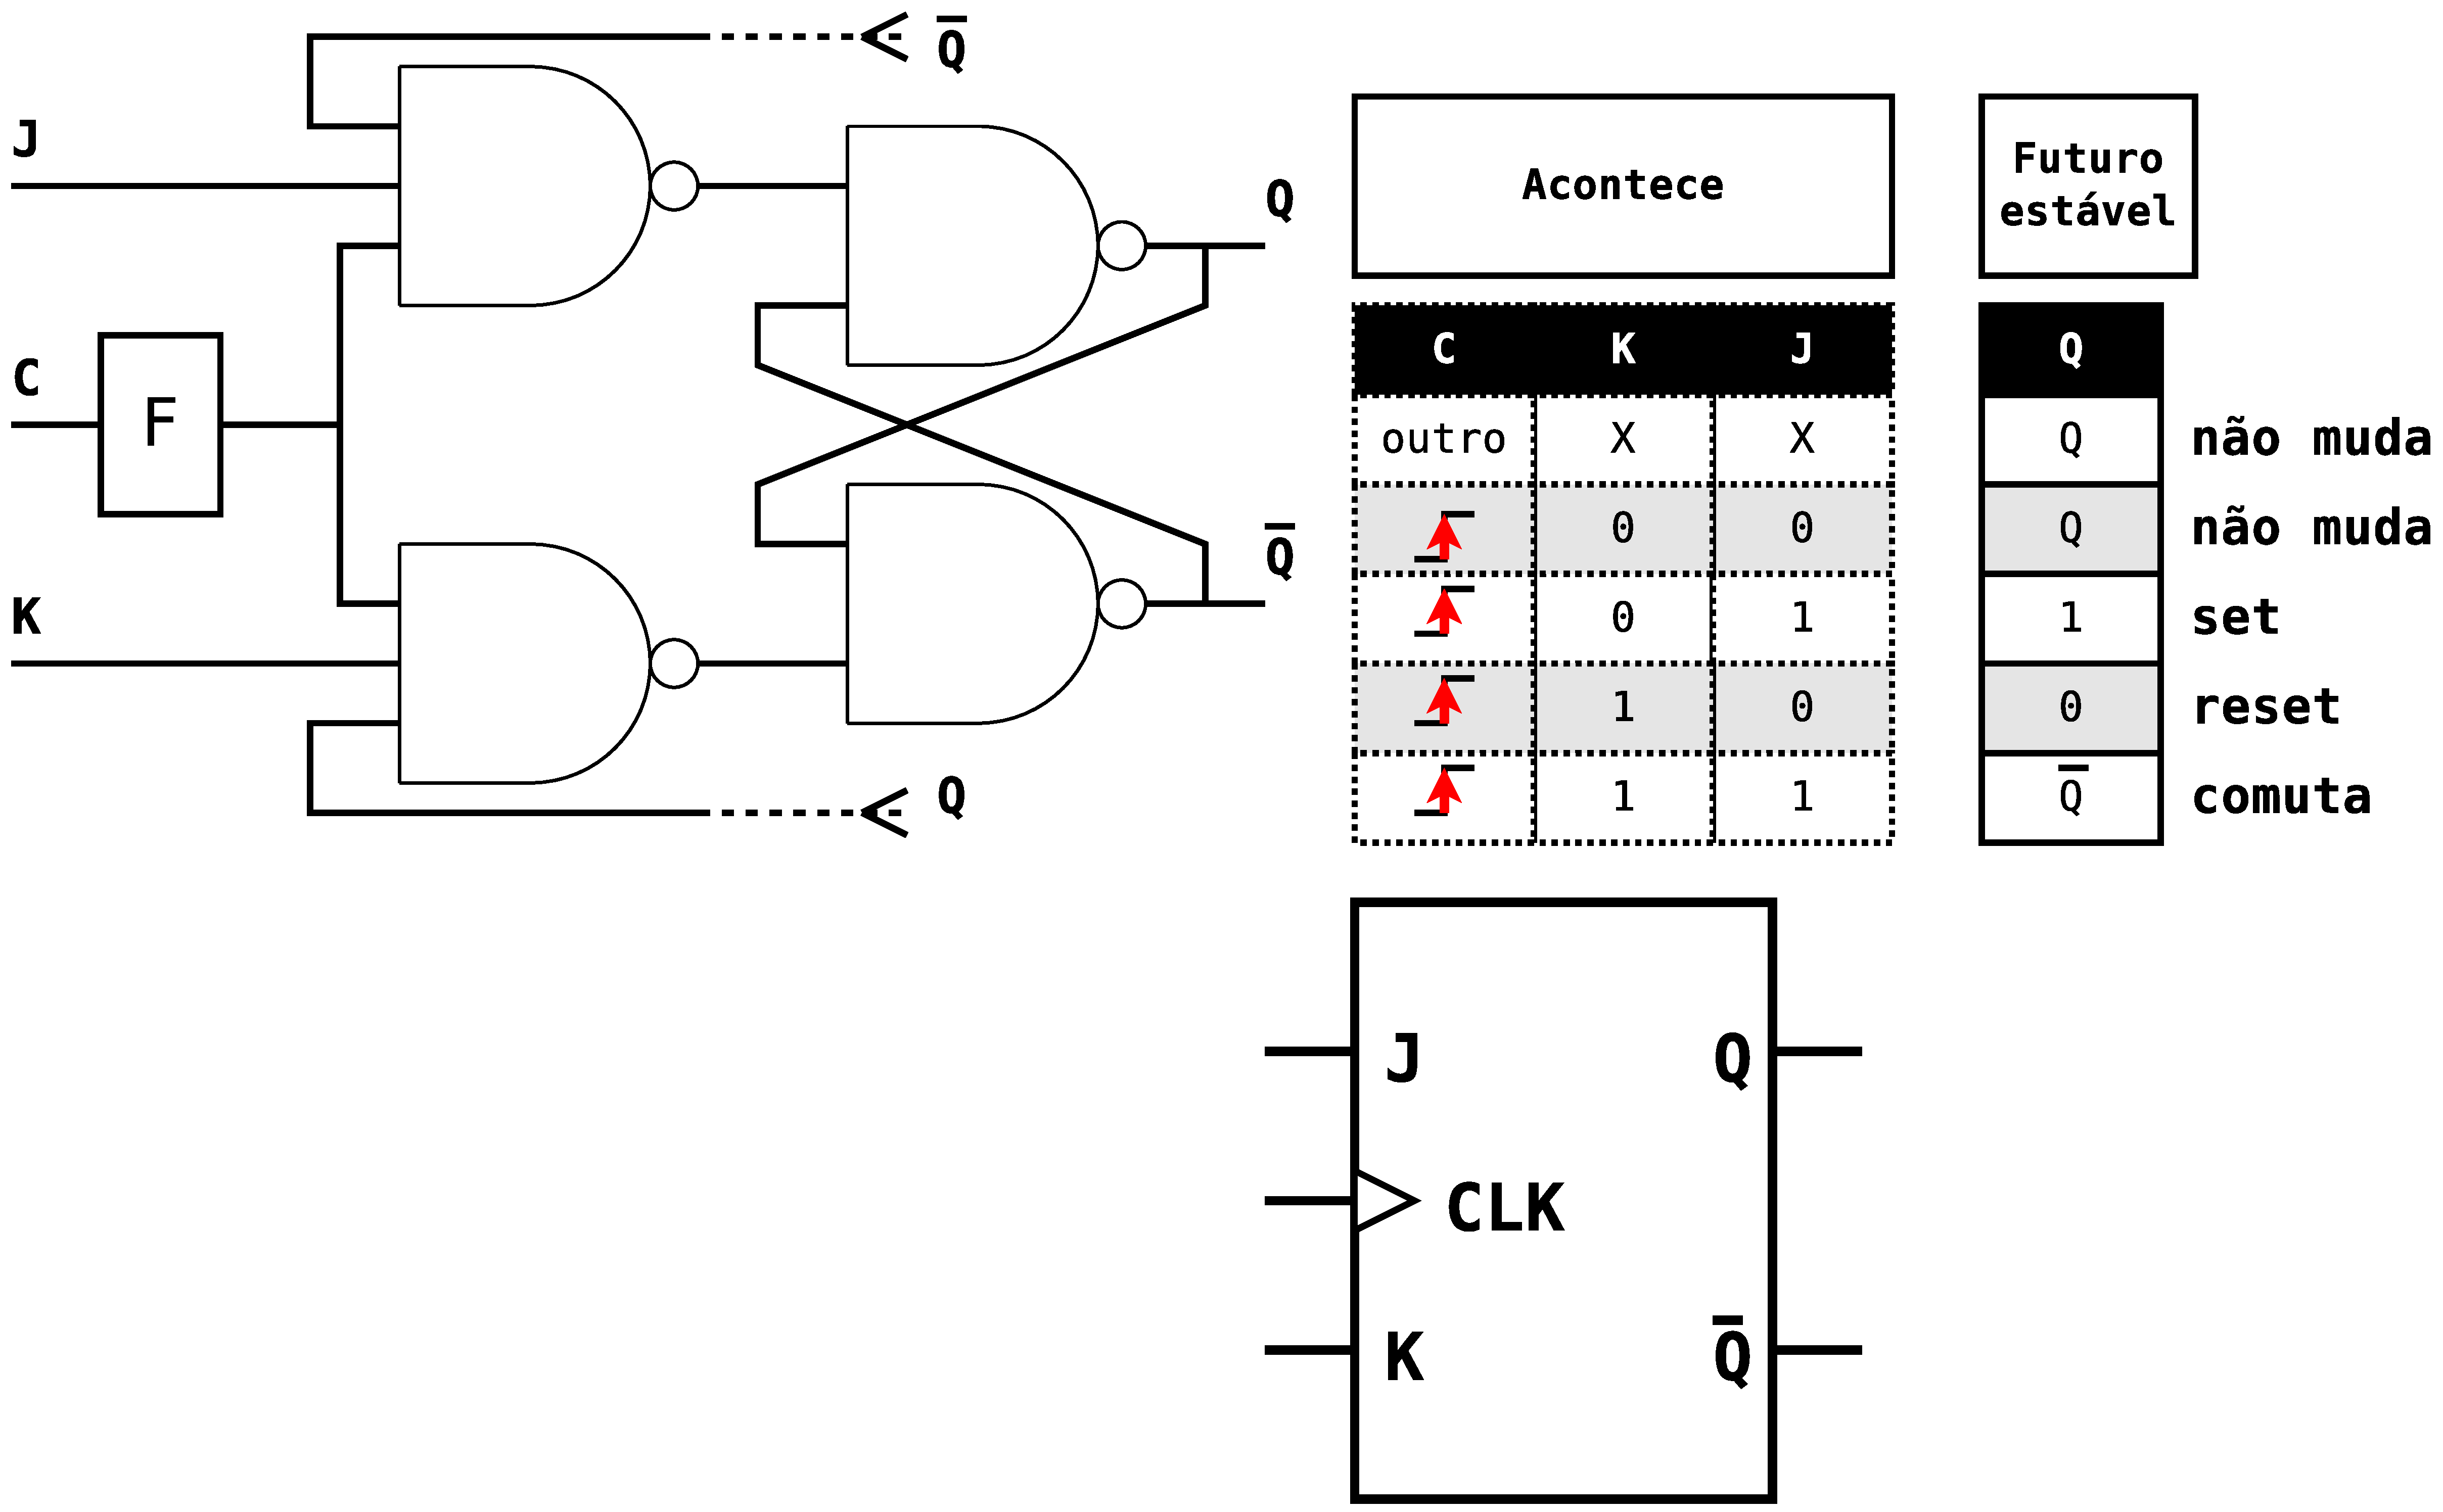
\includegraphics[width=0.99\textwidth]{images/jk.eps}
\end{center} 
\end{frame}


%%%%%%%%%%%%%%%%%%%%%%%%%%%%%%%%%%%%%%%%%%%%%%%%%%%%%%%%%%%%%%%%%%%%%%%%%%%%%%%%
\begin{frame}{Flip-Flop D}
\begin{center}
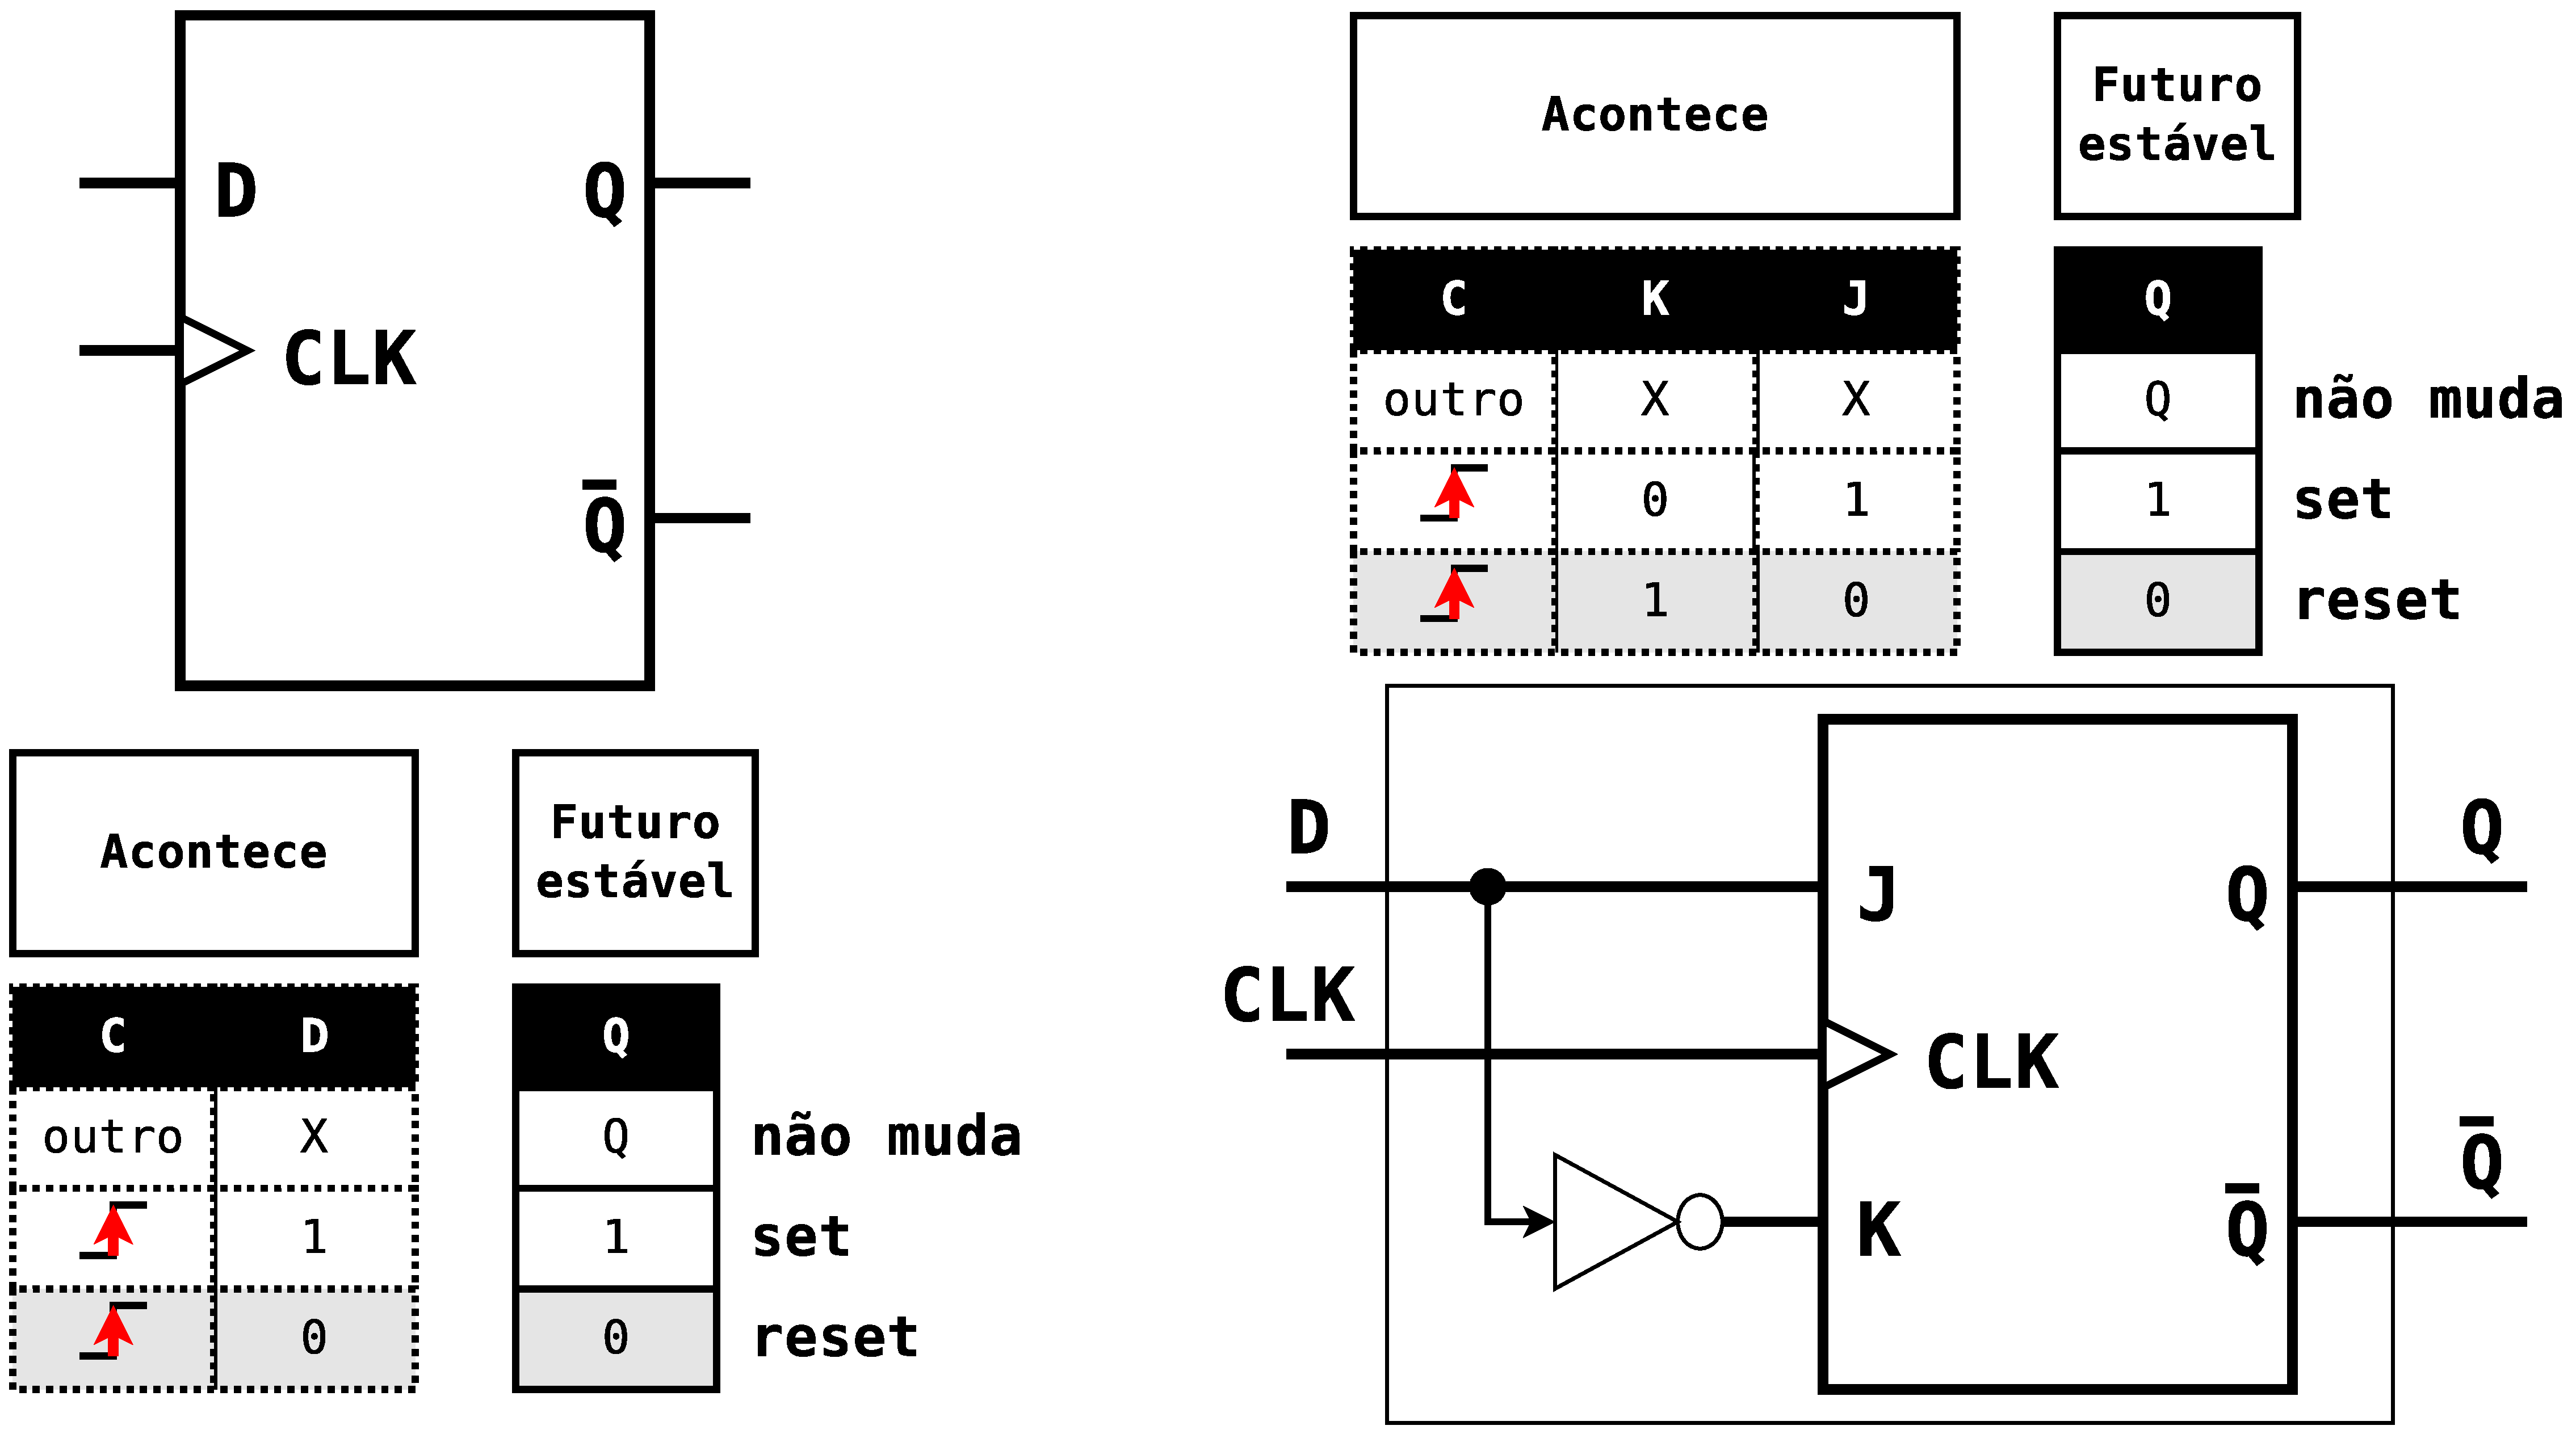
\includegraphics[width=0.99\textwidth]{images/dff.eps}
\end{center} 
\end{frame}

%%%%%%%%%%%%%%%%%%%%%%%%%%%%%%%%%%%%%%%%%%%%%%%%%%%%%%%%%%%%%%%%%%%%%%%%%%%%%%%%
\begin{frame}{Exemplo Flip-Flop JK - contador assíncrono}
\begin{center}
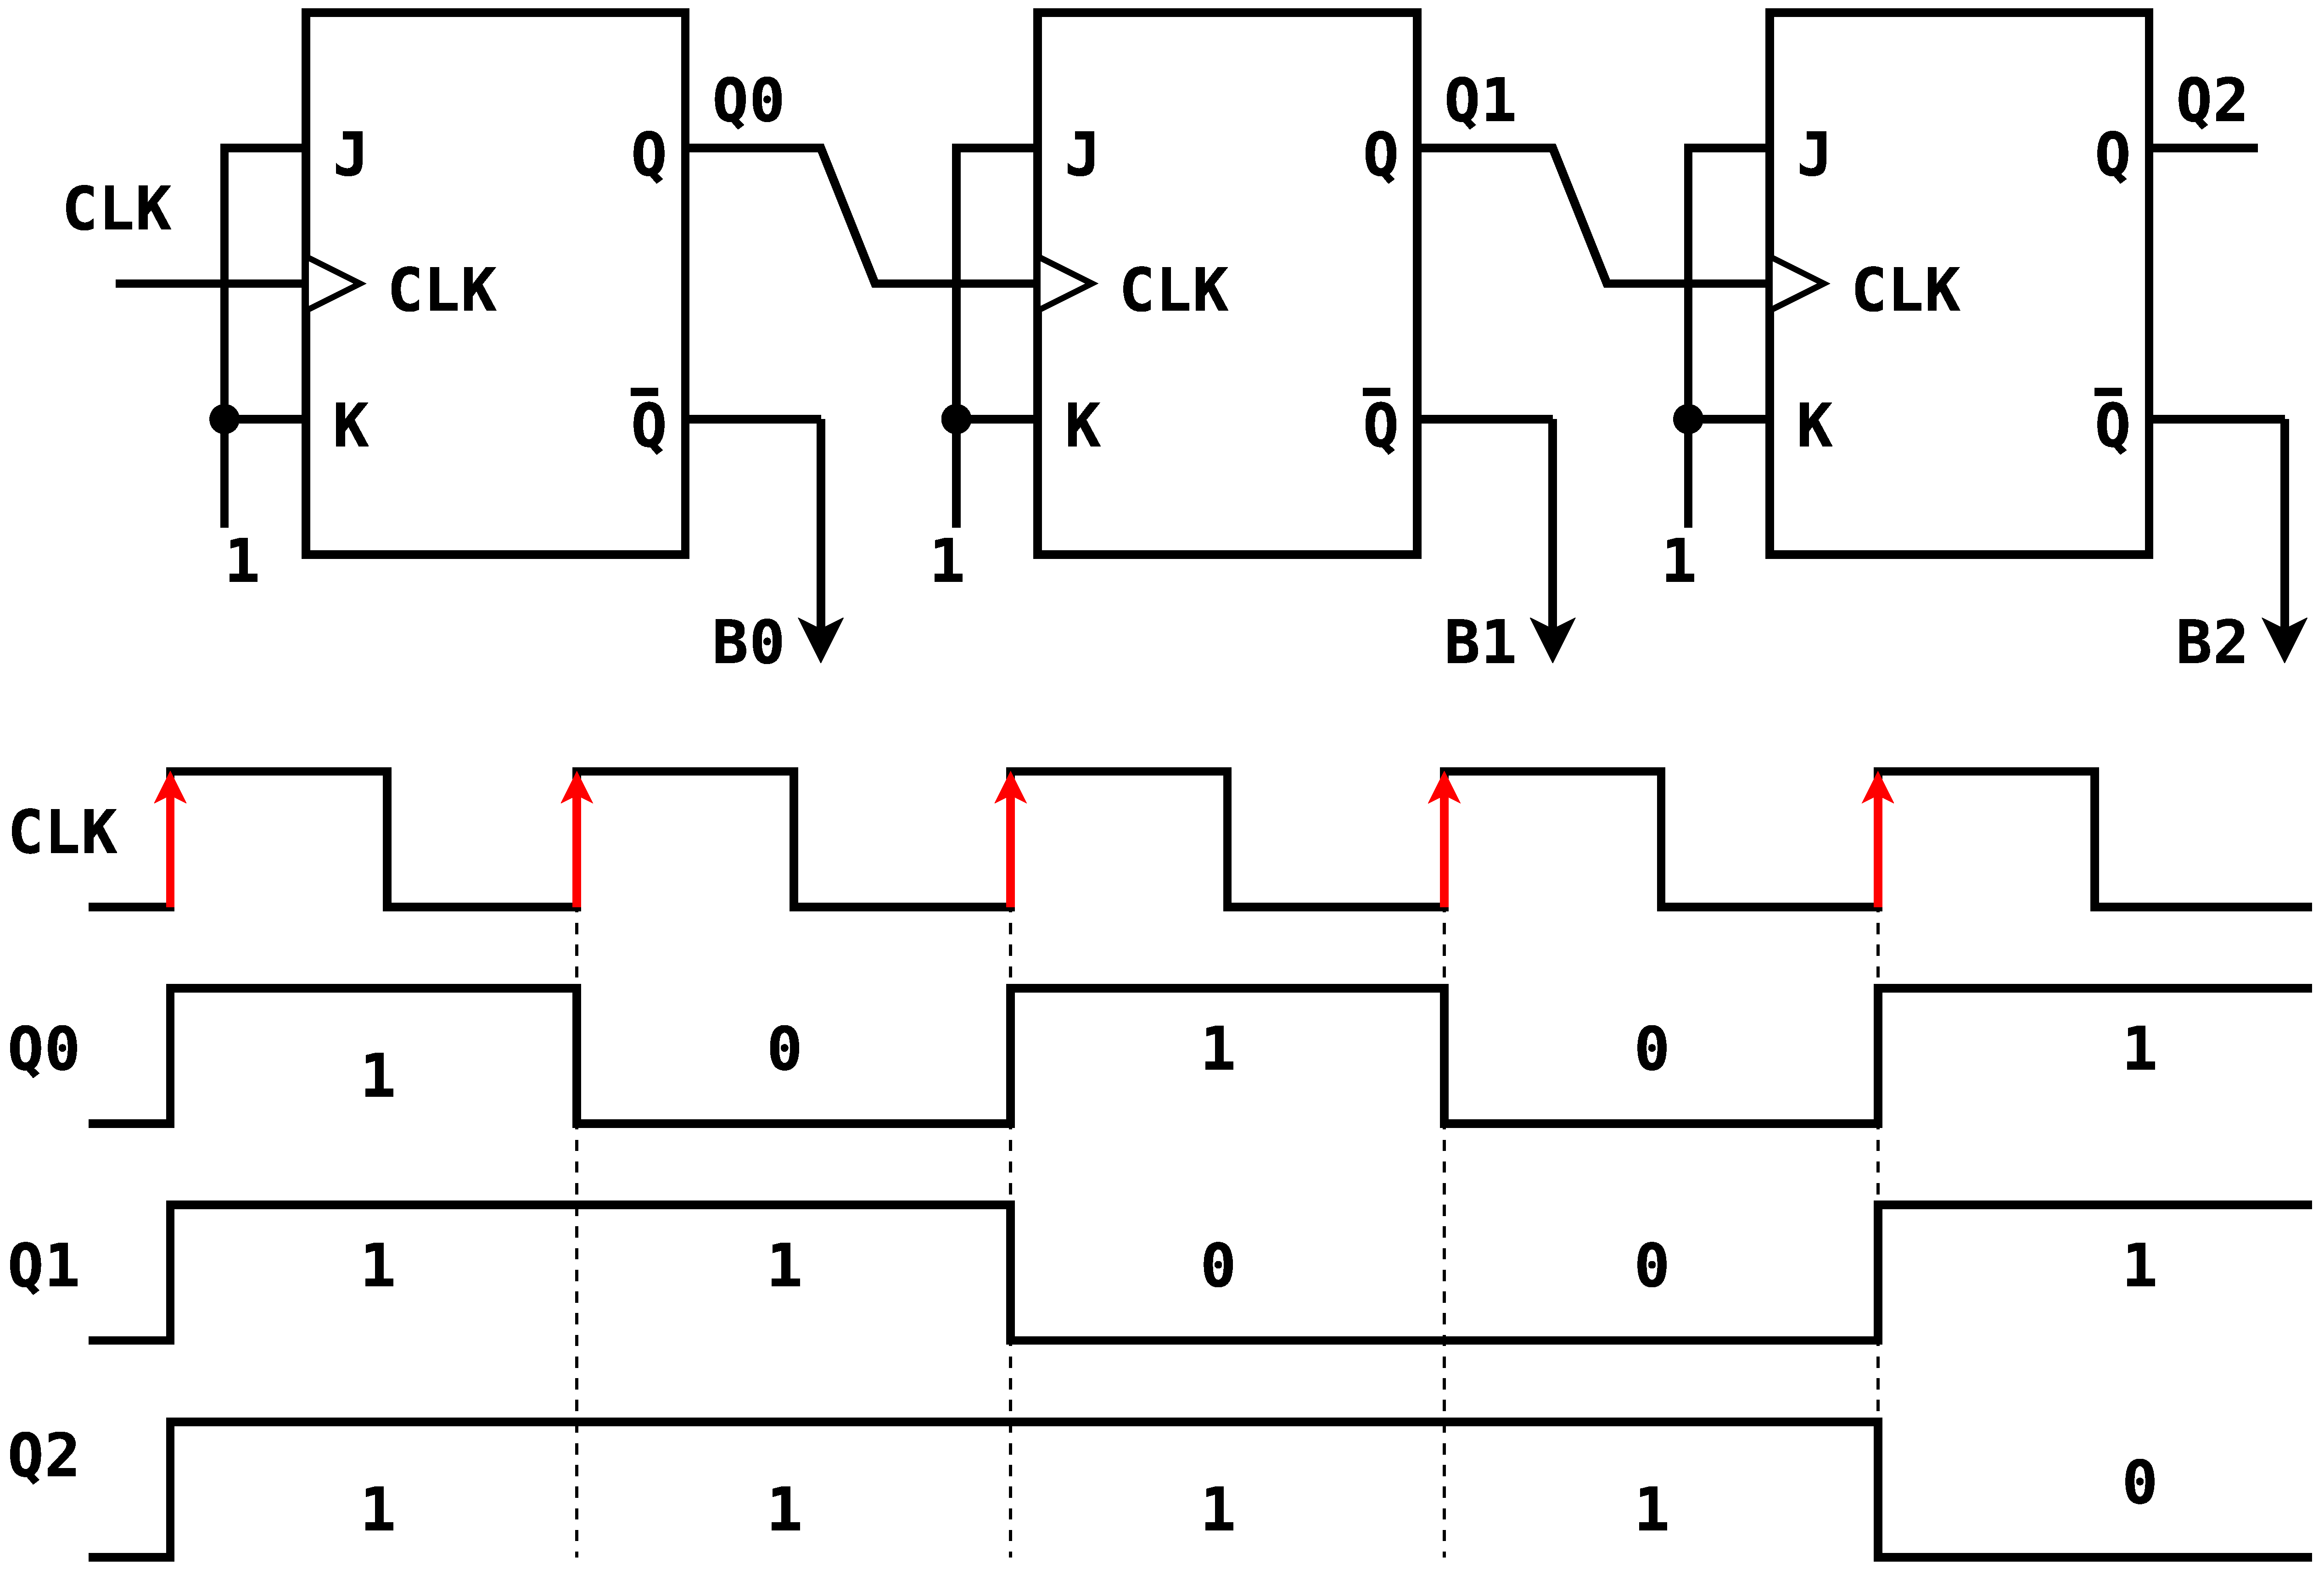
\includegraphics[width=0.8\textwidth]{images/ejemplojk.eps}
\end{center} 
\end{frame}

%%%%%%%%%%%%%%%%%%%%%%%%%%%%%%%%%%%%%%%%%%%%%%%%%%%%%%%%%%%%%%%%%%%%%%%%%%%%%%%%
\begin{frame}{Exemplo Flip-Flop JK - contador assíncrono}
\begin{center}
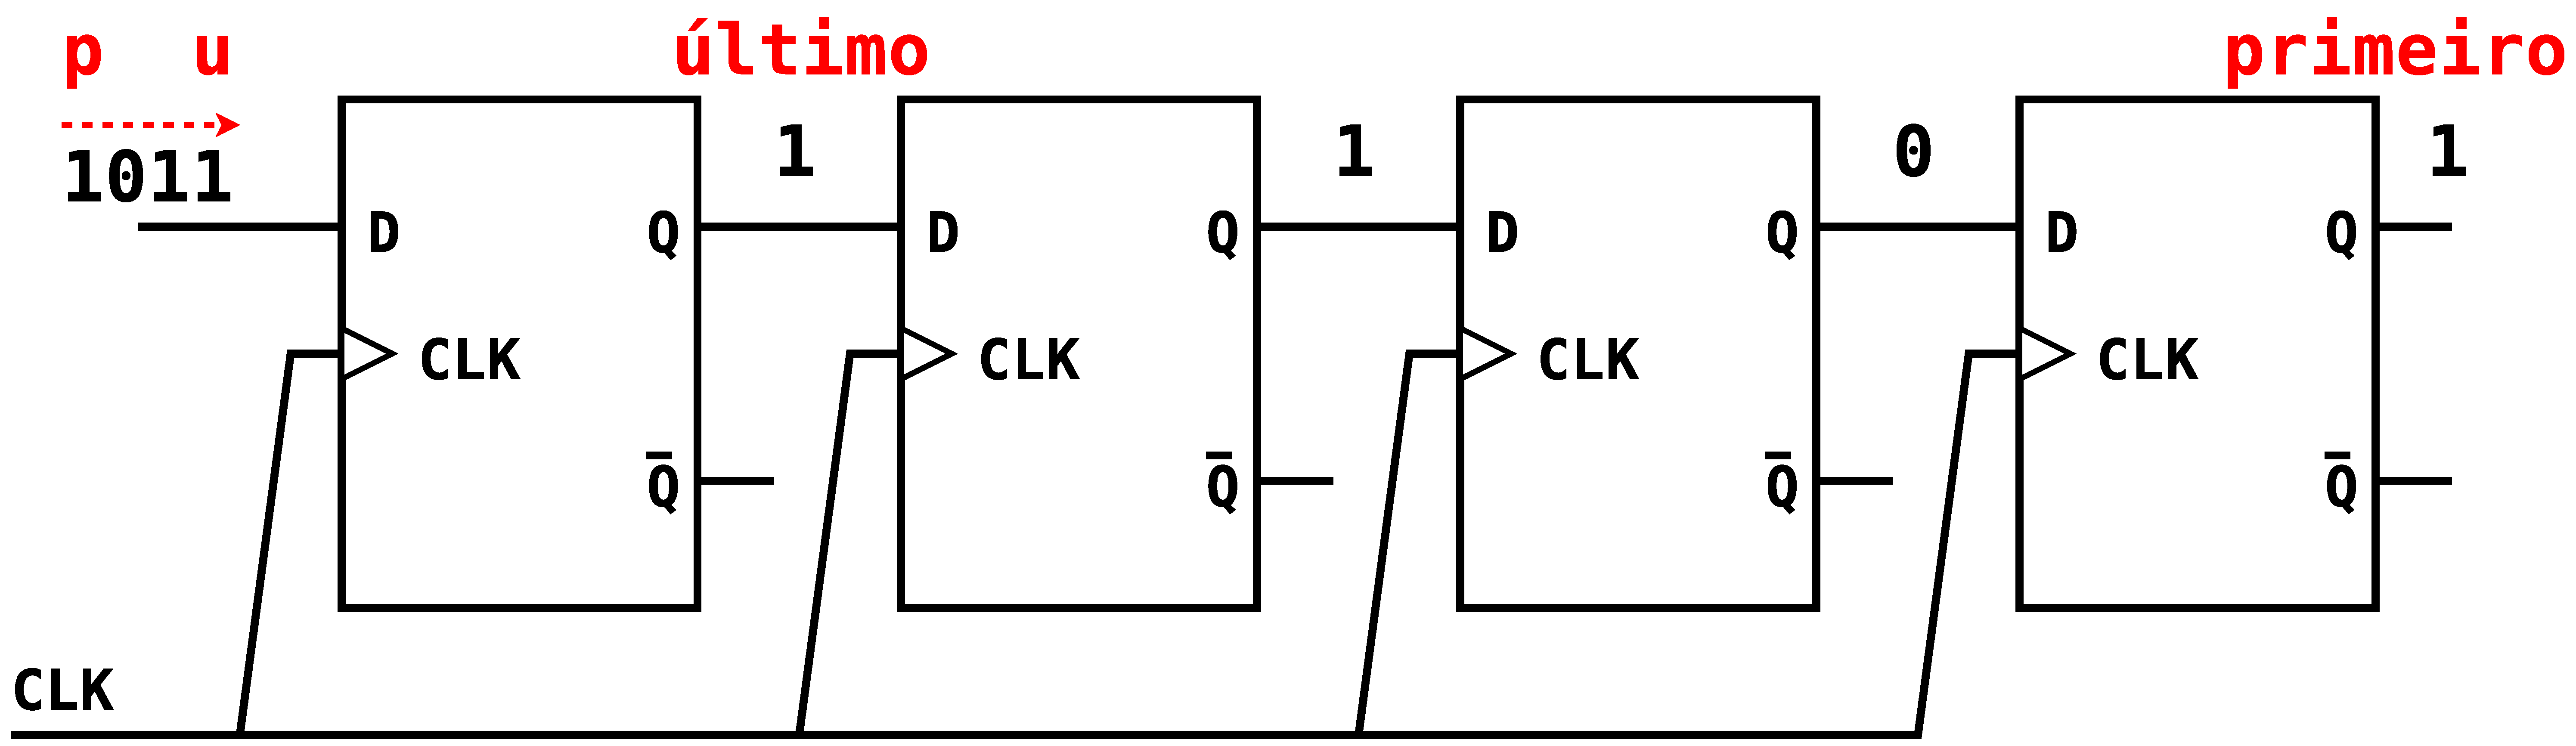
\includegraphics[width=0.8\textwidth]{images/ejemplod.eps}
\end{center} 
\end{frame}
%%%%%%%%%%%%%%%%%%%%%%%%%%%%%%%%%%%%%%%%%%%%%%%%%%%%%%%%%%%%%%%%%%%%%%%%%%%%%%%%
\begin{frame}[allowframebreaks]
        \frametitle{References}
        \bibliographystyle{plain}
\bibliography{sequencial}
\end{frame}



\end{document}
